% ============================================================
%  CHAPTER 3 — Methodology and Design
%  Harvard Dataset Crop Multi-Classification
%  Based on confirmed notebook outputs and project files
% ============================================================

\chapter{Methodology and Design}
\label{ch:method}

Accurate and timely crop type mapping is a critical component of modern
food security intelligence systems, yet it remains a persistent challenge
in smallholder farming landscapes such as Rwanda, where field sizes are
small, crop diversity is high, and cloud cover frequently limits satellite
observation. This chapter presents a rigorous, end-to-end methodology for
multi-class crop type mapping using Sentinel-2 multispectral time series
data and supervised machine learning — a pipeline designed not only to
produce high-quality classification outputs, but to do so in a way that
is reproducible, methodologically transparent, and operationally relevant
to the Rwanda Space Agency and the Ministry of Agriculture. The approach
combines field-collected ground truth data from the Harvard Dataverse with
Sentinel-2 imagery processed through a multi-stage quality control chain,
a rich feature engineering framework encompassing both statistical and
phenological descriptors, and a comparative model evaluation spanning
classical ensemble methods and deep learning sequence architectures. Each
methodological decision is grounded in physical reasoning, agronomic
context, or empirical evidence from the data, and is described in terms
of its purpose, inputs, outputs, and connection to subsequent stages.


% ============================================================
\section{Methodology Overview and Pipeline}
\label{sec:pipeline}
% ============================================================

Figure~\ref{fig:pipeline} provides a high-level schematic of the complete
methodology pipeline, from raw data acquisition to final model evaluation.

\begin{figure}[H]
\centering
\resizebox{\textwidth}{!}{%
\begin{tikzpicture}[
    font=\small,
    node distance=0.95cm and 0.9cm,
    stage/.style={
        rectangle,
        rounded corners=3pt,
        draw=#1!85!black,
        fill=#1!10,
        line width=0.8pt,
        minimum width=3.8cm,
        minimum height=0.9cm,
        align=center,
        text=chaptercolor,
        font=\small\bfseries
    },
    arrow/.style={
        -{Stealth[length=2.5mm]},
        line width=0.8pt,
        draw=accentgold!90!black
    },
    groupbox/.style={
        rounded corners=5pt,
        draw=#1!75!black,
        fill=#1!4,
        line width=0.9pt,
        inner sep=8pt
    },
    grouptext/.style={
        font=\small\bfseries,
        text=chaptercolor
    }
]

% ============================================================
% Row 1: Data and preprocessing
% ============================================================
\node[stage=accentgold] (data) {Ground Truth Polygons\\+ Sentinel-2 Time Series};
\node[stage=accentgold, right=of data] (schema) {Schema Validation\\+ Date Parsing};
\node[stage=accentgold, right=of schema] (season) {Season B Filter\\Feb--Aug 2025};
\node[stage=accentgold, right=of season] (dedup) {Duplicate Removal\\+ Zero-Band Check};

% ============================================================
% Row 2: Cleaning and quality control
% ============================================================
\node[stage=OliveGreen, below=1.35cm of dedup] (label) {Label Standardisation\\+ Monocrop Filtering};
\node[stage=OliveGreen, left=of label] (geometry) {Polygon Geometry QC\\Compactness Check};
\node[stage=OliveGreen, left=of geometry] (scaling) {Band and Quality Scaling\\Bands, AOT, CLP};
\node[stage=OliveGreen, left=of scaling] (quality) {Quality Masking\\SCL, AOT, CLP};

% ============================================================
% Row 3: Temporal reconstruction and features
% ============================================================
\node[stage=RoyalBlue, below=1.35cm of quality] (boundary) {Boundary Conflict Check\\Same-Date Multi-Label};
\node[stage=RoyalBlue, right=of boundary] (gap) {Gap Analysis\\+ Linear Interpolation};
\node[stage=RoyalBlue, right=of gap] (vi) {Vegetation Indices\\Greenness, Moisture, Red-Edge};
\node[stage=RoyalBlue, right=of vi] (features) {Feature Engineering\\Statistical + Phenological};

% ============================================================
% Row 4: Modelling
% ============================================================
\node[stage=BurntOrange, below=1.35cm of features] (split) {Train--Test Split\\QUADKEY + Field Check};
\node[stage=BurntOrange, left=of split] (select) {Feature Selection\\ANOVA+Bonferroni, RF, RFECV};
\node[stage=BurntOrange, left=of select] (imbalance) {Imbalance Strategy\\Top-3 Avg-Rank Selection};
\node[stage=BurntOrange, left=of imbalance] (models) {Benchmark + Top-3 Tuning\\Classical ML + Deep Learning};

% ============================================================
% Row 5: Evaluation and deployment
% ============================================================
\node[stage=BrickRed, below=1.35cm of models] (eval) {Evaluation\\Macro F1, PR-AUC, ROC, Confusion};
\node[stage=BrickRed, right=of eval] (robust) {Spatial Robustness\\Field/Group-Level Check};
\node[stage=BrickRed, right=of robust] (thresh) {Per-Class Threshold\\Calibration (Test)};
\node[stage=BrickRed, right=of thresh] (infer) {District-Scale Inference\\Dynamic World Mask};

% ============================================================
% Arrows
% ============================================================
\draw[arrow] (data) -- (schema);
\draw[arrow] (schema) -- (season);
\draw[arrow] (season) -- (dedup);

\draw[arrow] (dedup.south) -- (label.north);
\draw[arrow] (label) -- (geometry);
\draw[arrow] (geometry) -- (scaling);
\draw[arrow] (scaling) -- (quality);

\draw[arrow] (quality.south) -- (boundary.north);
\draw[arrow] (boundary) -- (gap);
\draw[arrow] (gap) -- (vi);
\draw[arrow] (vi) -- (features);

\draw[arrow] (features.south) -- (split.north);
\draw[arrow] (split) -- (select);
\draw[arrow] (select) -- (imbalance);
\draw[arrow] (imbalance) -- (models);

\draw[arrow] (models.south) -- (eval.north);
\draw[arrow] (eval) -- (robust);
\draw[arrow] (robust) -- (thresh);
\draw[arrow] (thresh) -- (infer);

% ============================================================
% Group boxes on background layer
% ============================================================
\begin{pgfonlayer}{background}
    \node[groupbox=accentgold, fit=(data)(schema)(season)(dedup),
          label={[grouptext]above:Data Preparation}] {};

    \node[groupbox=OliveGreen, fit=(quality)(scaling)(geometry)(label),
          label={[grouptext]above:Cleaning and Quality Control}] {};

    \node[groupbox=RoyalBlue, fit=(boundary)(gap)(vi)(features),
          label={[grouptext]above:Temporal Reconstruction and Feature Engineering}] {};

    \node[groupbox=BurntOrange, fit=(models)(imbalance)(select)(split),
          label={[grouptext]above:Model Development}] {};

    \node[groupbox=BrickRed, fit=(eval)(robust)(thresh)(infer),
          label={[grouptext]above:Evaluation and Inference}] {};
\end{pgfonlayer}

\end{tikzpicture}
}
\caption{End-to-end methodology pipeline for multi-class crop type mapping using Sentinel-2 time series and ground reference crop polygons.}
\label{fig:pipeline}
\end{figure}

Each block in Figure~\ref{fig:pipeline} corresponds to a dedicated subsection
in this chapter. The pipeline is strictly sequential: each stage receives
clean, validated output from the preceding stage, ensuring reproducibility and
traceability throughout the workflow. A fixed random seed (\texttt{RANDOM\_STATE~=~42})
is applied at every stochastic step to guarantee deterministic results.


% ============================================================
\section{Datasets}
\label{sec:datasets}
% ============================================================

Two ground-truth sources were considered during the project. The first was
provided through the Rwanda government and Oracle collaboration, but it
contained several data-quality issues that limited its suitability for the
final modelling workflow. For this reason, the final report
focuses on the Harvard Dataverse Rwanda crop mapping dataset, which provides
the ground-truth labels used for the methodology described in this chapter.

The Harvard dataset was spatially joined with Sentinel-2 time series by the
data engineering team, producing the QUADKEY-indexed dataset used throughout
this work.


% ------------------------------------------------------------
\subsection{Harvard Dataverse Rwanda Crop Mapping Dataset}
\label{subsec:harvard}
% ------------------------------------------------------------

The primary dataset used in this study is the Rwanda Crop Mapping Ground
Truth dataset published on Harvard Dataverse~\cite{harvard2025}. It was
collected between 6~May~2025 and 7~June~2025 in support of a remote
sensing-based crop monitoring system funded by GIZ~Rwanda and implemented
by the Alliance of Bioversity and CIAT under the supervision of the Rwanda
Space Agency and the Ministry of Agriculture and Animal Resources
(MinAgri)~\cite{harvard2025}.

The dataset covers four administrative districts: Nyagatare, Ruhango,
Musanze, and Nyabihu. Field enumerators collected crop observations using
the KoBo~Toolbox platform, recording GPS-referenced points with attribute
photographs (field pictures, attributes F15/F15a). Homogeneous field
polygons were then delineated around pixels representing particular crop
types using satellite imagery. The geographic projection is WGS84.

The raw Harvard dataset contains labelled field polygons for multiple crop
types, including both monocrop and intercrop entries. In the Sentinel-2
joined dataset used for modelling, the classification target is the textual
\texttt{landcover} column. This column is standardised and then filtered to
retain only the four monocrop classes used in this study, as described in
Section~\ref{subsec:label_std}. When joined with Sentinel-2 time series at
zoom level~22, the raw dataset contains 1,788,552 observations across
27 columns.

\subsubsection*{Season B Alignment}
\label{subsubsec:seasonb}

Temporal filtering to the Season~B window (February through August) is
applied immediately after data loading because the dataset documentation
explicitly states that ground-truth collection targeted Season~B~2025.
Retaining observations outside this agronomic window would introduce
phenological noise from other seasons and risk mislabelling pixels that
do not correspond to the intended crop growth cycle. This filter is
therefore a direct methodological requirement imposed by the dataset's
collection context, not an arbitrary choice.


% ------------------------------------------------------------
\subsection{Dataset Schema and Column Descriptions}
\label{subsec:schema}
% ------------------------------------------------------------

The raw Sentinel-2 joined dataset contains spectral signal columns,
quality flags, spatial and temporal metadata, polygon identifiers, and
the crop label used as the classification target. The full
column-by-column schema is provided in Appendix~\ref{app:detailed_methodology_tables}
(Table~\ref{tab:columns}) to keep the main methodology chapter focused on
the processing workflow.


% ------------------------------------------------------------
\subsubsection{Sentinel-2 Scene Classification Layer (SCL)}
\label{subsubsec:scl}
% ------------------------------------------------------------

The Scene Classification Layer (SCL) is a per-pixel quality assessment
product generated automatically by the Sentinel-2 Level-2A processing
chain (Sen2Cor)~\cite{mainknorn2017sen2cor}. It assigns each pixel to one
of twelve land surface or atmospheric categories based on spectral
thresholds and spatial context. The full SCL class definitions are
reported in Appendix~\ref{app:detailed_methodology_tables}
(Table~\ref{tab:scl}).

Only SCL classes 4 (Vegetation) and 5 (Bare Soils) are defined as
acceptable in this study (\texttt{GOOD\_SCL} = (4,~5)). This choice is
grounded in the modelling objective: crop classification requires
observations that correspond to actual land surfaces, free from
atmospheric and sensor contamination. Pixels classified as clouds, cloud
shadows, water, or defective are spectrally unreliable and would introduce
systematic noise into the time series if retained.

Observations failing the SCL test are not immediately removed from the
dataset. Instead, their spectral band values are set to \texttt{NaN},
preserving the regular 7-day temporal grid of each QUADKEY's time series.
This enables subsequent linear interpolation to recover plausible spectral
values at masked timesteps (see Section~\ref{subsec:interpolation}).
Removing rows outright would create irregular time series incompatible
with phenological feature extraction.


% ------------------------------------------------------------
\subsection{Band Value Scaling and Normalisation}
\label{subsec:scaling}
% ------------------------------------------------------------

Raw Sentinel-2 Level-2A products store surface reflectance as scaled
integers (Digital Numbers, DNs) rather than physical reflectance values.
Scaling to physical units is a mandatory preprocessing step for two
reasons: (1)~it ensures that spectral values are interpretable in physical
terms (reflectance in $[0,1]$), and (2)~it ensures feature-scale
consistency, which is critical for distance-based models, gradient-based
optimisers in deep learning, and any cross-band arithmetic operation
(e.g., vegetation index computation).

Three scaling operations are applied, each with a distinct physical
justification:

\paragraph{Sentinel-2 spectral bands (B01--B12, B8A):}
\begin{equation}
\label{eq:band_scale}
R_{\lambda} = \frac{\mathrm{DN}_{\lambda}}{10{,}000}
\end{equation}
Sentinel-2 Level-2A products encode surface reflectance with a
quantisation factor of 10{,}000: a true reflectance of 1.0 is stored as
the integer 10{,}000, and 0.5 as 5{,}000. Dividing by 10{,}000 converts
each band into its true reflectance value in the range $[0,1]$. This is
the standard convention documented in the Sentinel-2 product
specification~\cite{esa2021s2}.

\paragraph{Aerosol Optical Thickness (AOT):}
\begin{equation}
\label{eq:aot_scale}
\mathrm{AOT}_{\text{scaled}} = \frac{\mathrm{AOT}_{\text{DN}}}{1{,}000}
\end{equation}
The AOT column is encoded as an integer with a scale factor of 1{,}000,
consistent with the Sentinel-2 Level-2A product encoding for atmospheric
parameters. Dividing by 1{,}000 recovers the physical aerosol optical
depth at 550~nm. Values above 0.3 after scaling indicate elevated aerosol
loading, which degrades surface reflectance retrieval quality.

\paragraph{Cloud Probability (CLP):}
\begin{equation}
\label{eq:clp_scale}
\mathrm{CLP}_{\text{scaled}} = \frac{\mathrm{CLP}_{\text{DN}}}{255}
\end{equation}
The CLP column is an 8-bit unsigned integer ranging from 0 to 255,
where 255 represents 100\% cloud probability. Dividing by 255 maps it to
the $[0,1]$ range, consistent with the standard normalisation of 8-bit
pixel values. Thresholding at 0.4 after scaling identifies observations
with a cloud probability exceeding 40\%.


% ============================================================
\section{QUADKEY Spatial Tiling and Zoom Level~22}
\label{sec:quadkey}
% ============================================================

The dataset represents each ground observation as a QUADKEY tile — a
string identifier from Microsoft's Bing Maps tiling system that encodes
both the spatial location and the hierarchical zoom level of a square
tile on the Earth's surface~\cite{bing2010}. QUADKEYs are used at
\textbf{zoom level~22} in this study.

The ground resolution of a QUADKEY tile at a given zoom level $z$ and
geographic latitude $\phi$ is given by:
\begin{equation}
\label{eq:ground_res}
r = \frac{156{,}543.034 \times \cos\phi}{2^{z}} \quad \text{(metres per pixel)}
\end{equation}
At zoom level~22 and Rwanda's mean latitude of approximately $\phi \approx
-1.9°$:
\begin{equation}
r \approx \frac{156{,}543.034 \times \cos(-1.9°)}{2^{22}}
  \approx \frac{156{,}543.034 \times 0.9994}{4{,}194{,}304}
  \approx 9.55 \approx 10 \text{ m/pixel}
\end{equation}

This result is not a coincidence: zoom level~22 was chosen because it
produces a ground resolution of approximately 10~metres, matching the
native spatial resolution of the core Sentinel-2 optical bands
(B02--B08). This alignment allows the QUADKEY to act as the spatial unit
of analysis for linking ground-truth polygons with Sentinel-2 observations.
Each QUADKEY therefore represents a consistent spatial tile across the
Season~B time series, making it suitable for temporal feature extraction
and crop classification.


% ============================================================
\section{Data Preprocessing and Quality Control}
\label{sec:preprocessing}
% ============================================================

Data preprocessing follows a strict, ordered pipeline in which each step
addresses a specific data quality issue and produces a cleaner dataset
for the subsequent stage. Steps are applied in the following sequence:
schema validation, temporal filtering, full-row deduplication, zero-band
detection, label standardisation and monocrop filtering, polygon geometry
quality control, band scaling, temporal deduplication, spectral quality
nullification (SCL/AOT/CLP), boundary pixel removal, and finally gap
analysis with linear interpolation.


% ------------------------------------------------------------
\subsection{Schema Validation and Date Parsing}
\label{subsec:schema_val}
% ------------------------------------------------------------

The first step verifies that all columns required by the downstream
pipeline are present in the loaded dataset. A \texttt{ValueError} is
raised immediately if any expected column is missing, ensuring that
downstream failures cannot occur silently due to schema changes in the
data source. The \texttt{START\_DATE} and \texttt{END\_DATE} columns are
parsed from string format to \texttt{datetime64[ns]}, enabling all
subsequent temporal operations (filtering, sorting, differencing,
and ISO week extraction).


% ------------------------------------------------------------
\subsection{Temporal Filtering to Season~B}
\label{subsec:temporal_filter}
% ------------------------------------------------------------

Observations are filtered to retain only those with a \texttt{START\_DATE}
falling within calendar months 2 through 8 (February to August,
inclusive). As established in Section~\ref{subsec:harvard}, this window
corresponds directly to Rwanda's Season~B crop growing cycle and matches
the ground-truth collection context documented in the dataset metadata.

Retaining out-of-season observations (September to January) would
introduce spectral signals from a different agricultural state than what
the field labels represent. A maize field labelled in June during active
vegetative growth would appear spectrally very different in December after
harvest; combining such observations would corrupt the feature distribution
and degrade classification performance. Two derived columns are added at
this stage: \texttt{year} (ISO calendar year) and \texttt{week} (ISO
calendar week number), both cast to \texttt{int16} for memory efficiency.
After filtering, the dataset contains 1,490,460 observations covering
27,093 unique QUADKEYs, spanning 2025-02-05 to 2025-08-27.


% ------------------------------------------------------------
\subsection{Full-Row Duplicate Removal}
\label{subsec:dedup_full}
% ------------------------------------------------------------

A duplicate check reveals that 502,800 rows (33.7\% of the temporally
filtered dataset) are exact duplicates across all columns. Full-row
duplicates arise from the data pipeline used to join ground-truth polygons
with Sentinel-2 tiles: when a field polygon overlaps multiple tile export
boundaries, the same pixel observation can be delivered twice with
identical attribute values. Retaining duplicates would artificially
inflate the apparent dataset size, introduce correlated samples into
cross-validation folds, and bias model training toward over-represented
spatial regions.

All duplicate rows are removed, reducing the dataset from 1,490,460 to
987,660 rows. The duplicate check is performed at the full-row level
rather than on a key subset, to avoid removing legitimate observations
that share only a partial key but differ in spectral content.


% ------------------------------------------------------------
\subsection{Zero-Band Row Detection and Removal}
\label{subsec:zero_band}
% ------------------------------------------------------------

Rows in which all spectral band columns (B01--B12) simultaneously equal
zero are physically invalid. A Sentinel-2 observation with zero
reflectance across all bands indicates a sensor failure, a no-data fill
value incorrectly recorded as zero, or a corrupted pixel. Such rows
cannot be imputed because their spectral content is entirely absent, and
their inclusion in the training set would introduce a degenerate signal
that could mislead the classifier. All such rows are identified and
removed before any further processing.


% ------------------------------------------------------------
\subsection{Label Standardisation and Monocrop Filtering}
\label{subsec:label_std}
% ------------------------------------------------------------

The \texttt{landcover} column is standardised by converting all values to
uppercase, stripping leading and trailing whitespace, and collapsing
internal consecutive whitespace to a single space. This step ensures that
semantically identical labels such as \texttt{"maize"}, \texttt{"Maize"},
and \texttt{"MAIZE"} are treated as a single class.

Following standardisation, the dataset contains 12 distinct label
categories, of which 8 describe intercropping or mixed-crop systems
(e.g., \texttt{BEAN AND MAIZE}, \texttt{BEAN, MAIZE, AND PUMPKIN}). This
study targets monocrop classification; mixed-crop pixels are excluded
because their spectral signal is a superposition of multiple crop
phenologies and cannot be reliably assigned to a single label. Mixed-crop
labels are identified by a regular expression pattern that detects the
keyword \texttt{AND} at a word boundary or a comma
($\texttt{r"}\backslash\texttt{bAND}\backslash\texttt{b|},$"), and all
matching rows are removed.

After filtering, four monocrop classes are retained:
\textbf{MAIZE}, \textbf{RICE}, \textbf{BEAN}, and \textbf{IRISH POTATO}.
The dataset is reduced from 987,660 to 830,940 rows, and from 27,093 to
23,339 unique QUADKEYs.


% ------------------------------------------------------------
\subsection{Polygon Geometry Quality Control}
\label{subsec:compactness}
% ------------------------------------------------------------

A polygon compactness check is included as a diagnostic geometry-quality
control step. This check was motivated by earlier work with the Oracle/Rwanda
government ground-truth dataset, where several field polygons were found to
be highly elongated or geometrically irregular. Such polygons can intersect
many boundary pixels and may produce ambiguous QUADKEY labels after spatial
joining with Sentinel-2. Although the final report focuses on the Harvard
Dataverse dataset, the same compactness diagnostic was retained to verify
that similar geometry-quality problems were not present in the Harvard
polygons.

Polygon compactness is quantified using the \textbf{Polsby--Popper}
measure~\cite{polsbypopper1991}, a widely used geometric index that
returns values close to zero for elongated or irregular shapes and
approaches unity for a perfect circle. The raw compactness score is
defined as:
\begin{equation}
\label{eq:compactness}
C = \frac{A}{P^{2}}
\end{equation}
where $A$ is the polygon area (in projected units$^{2}$) and $P$ is its
perimeter. The isoperimetric (normalised) Polsby--Popper score, which
evaluates to 1 for a circle, is obtained by:
\begin{equation}
\label{eq:compactness_iso}
C_{\mathrm{PP}} = 4\pi \cdot C = \frac{4\pi A}{P^{2}}
\end{equation}
Both $C$ and $C_{\mathrm{PP}}$ are computed for each unique WKT polygon.
A polygon is flagged as suspicious if it is geometrically invalid
(\texttt{is\_valid = False}) or if its raw compactness score falls below
the threshold $C < 0.01$. A polygon compactness distribution histogram
is produced as a diagnostic figure (Figure~\ref{fig:compactness}).

In the Harvard dataset, this check is used primarily as a validation step.
It documents polygon geometry quality and confirms whether low-compactness
polygons need to be removed before modelling.

\begin{figure}[H]
    \centering
    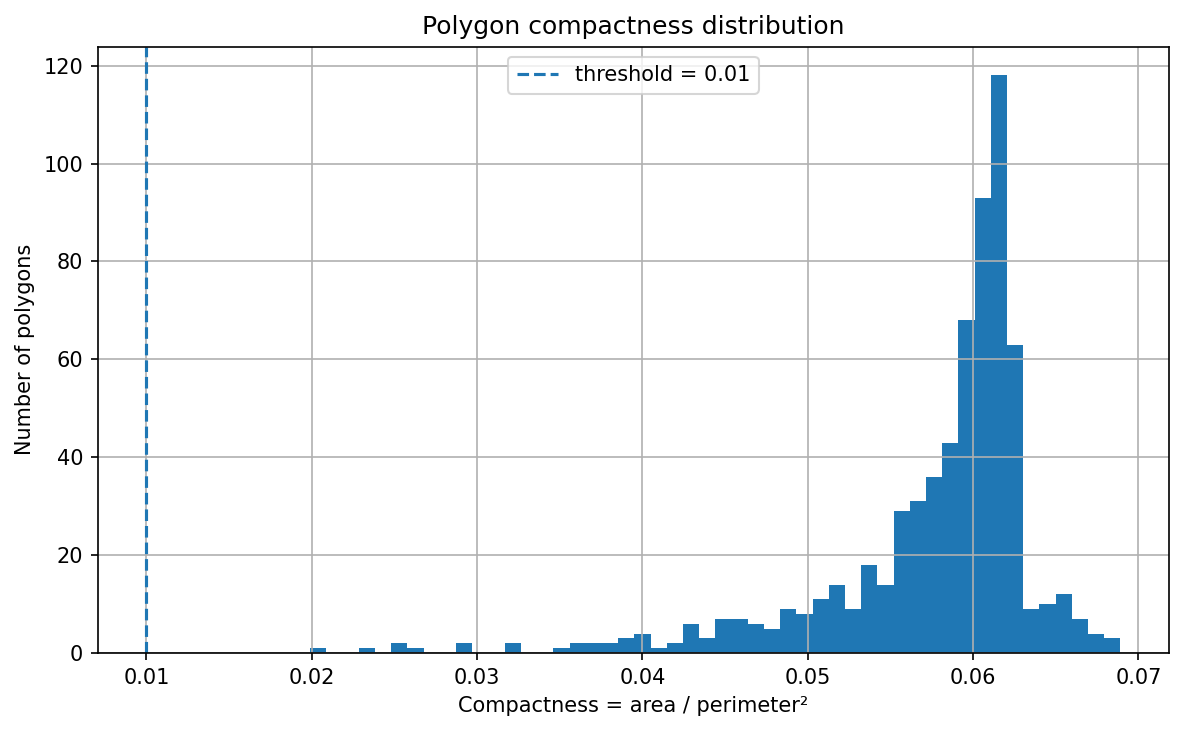
\includegraphics[width=\textwidth]{figures/polygon_compactness_distribution.png}
    \caption{Distribution of polygon compactness scores ($C = A/P^{2}$)
    across all 669 unique WKT field polygons. The dashed vertical line
    marks the low-compactness threshold at $C = 0.01$.}
    \label{fig:compactness}
\end{figure}


% ------------------------------------------------------------
\subsection{Band Scaling}
\label{subsec:scaling_step}
% ------------------------------------------------------------

Band scaling is applied after label filtering and geometry quality control,
and \emph{before} temporal deduplication. This ordering is deliberate:
deduplication selects the best observation per week using AOT and CLP as
ranking criteria, and those criteria must be evaluated in their scaled
(physically meaningful) form to ensure that the thresholds are correctly
applied. Scaling equations and their physical justifications are given in
Section~\ref{subsec:scaling}.


% ------------------------------------------------------------
\subsection{Temporal Deduplication: Best Observation Per Week}
\label{subsec:temporal_dedup}
% ------------------------------------------------------------

After full-row deduplication (Section~\ref{subsec:dedup_full}), a further
130,680 duplicate combinations of (\texttt{QUADKEY}, \texttt{START\_DATE},
\texttt{Landcover}) remain. These arise from overlapping Sentinel-2
satellite passes: the same tile can be observed by multiple orbits within
a 7-day compositing window, producing multiple valid observations for the
same location and date. Rather than arbitrarily discarding one, the
pipeline retains the \emph{highest-quality} observation using a
multi-criteria ranking.

Each observation is ranked by the following criteria in priority order:
\begin{enumerate}
    \item \textbf{SCL class}: observations whose SCL value is in
          \texttt{GOOD\_SCL} = \{4, 5\} are ranked first;
    \item \textbf{AOT} (ascending): lower aerosol loading is preferred;
    \item \textbf{CLP} (ascending): lower cloud probability is preferred.
\end{enumerate}
Within each (\texttt{QUADKEY}, \texttt{START\_DATE}, \texttt{Landcover})
group, the dataset is sorted by these criteria and the first row is kept,
leaving zero remaining duplicates on the key subset.

The rationale for preferring a quality-ranking strategy over simple
averaging is that Sentinel-2 surface reflectance values from cloudy or
aerosol-contaminated observations are systematically biased. Averaging
a cloud-free and a cloud-contaminated observation would produce a
spectrally compromised composite that is worse than the cloud-free
observation alone.


% ------------------------------------------------------------
\subsection{Spectral Quality Nullification (SCL, AOT, and CLP Masking)}
\label{subsec:nullification}
% ------------------------------------------------------------

Following temporal deduplication, a quality-control step sets the spectral
values of observations that fail any of the following three criteria to
\texttt{NaN}:

\begin{enumerate}
    \item $\mathrm{AOT}_{\text{scaled}} > 0.3$ (aerosol loading too high);
    \item $\mathrm{CLP}_{\text{scaled}} > 0.4$ (cloud probability too high);
    \item $\mathrm{SCL} \notin \{4, 5\}$ (non-vegetation, non-bare-soil pixel).
\end{enumerate}

Observations failing one or more criteria have all spectral band values
set to \texttt{NaN}. The row is retained, but its spectral content is
treated as missing. This preserves the regular 7-day temporal grid of
each QUADKEY's time series, which is required for consistent gap analysis
and linear interpolation. Three diagnostic plots are generated at this
stage (Figure~\ref{fig:qc_plots}): the AOT distribution with threshold
marker, the CLP distribution with threshold marker, and the SCL class
frequency bar chart with the accepted classes highlighted.

\begin{figure}[H]
    \centering
    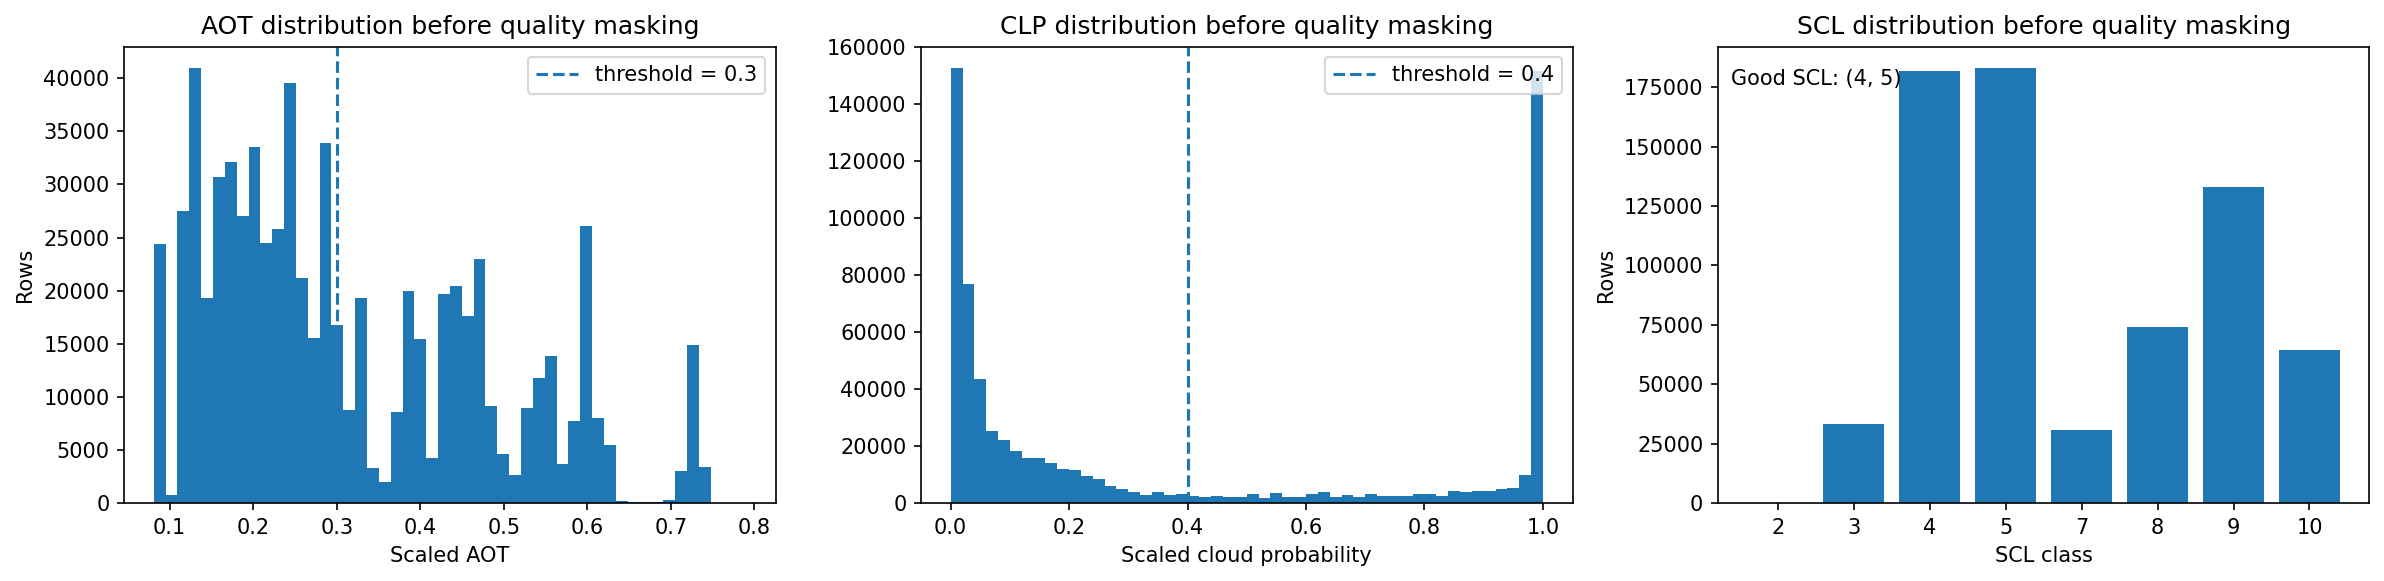
\includegraphics[width=\textwidth]{figures/quality_inputs_aot_clp_scl.png}
    \caption{Quality-control diagnostic plots for AOT, CLP, and SCL
    distributions after temporal deduplication but before spectral
    nullification. Vertical dashed lines indicate the applied thresholds.}
    \label{fig:qc_plots}
\end{figure}

Additionally, a temporal quality plot shows the percentage of
nullified observations per acquisition date across the Season~B window,
revealing strong temporal variability in cloud cover
(Figure~\ref{fig:lq_by_date}).

\begin{figure}[H]
    \centering
    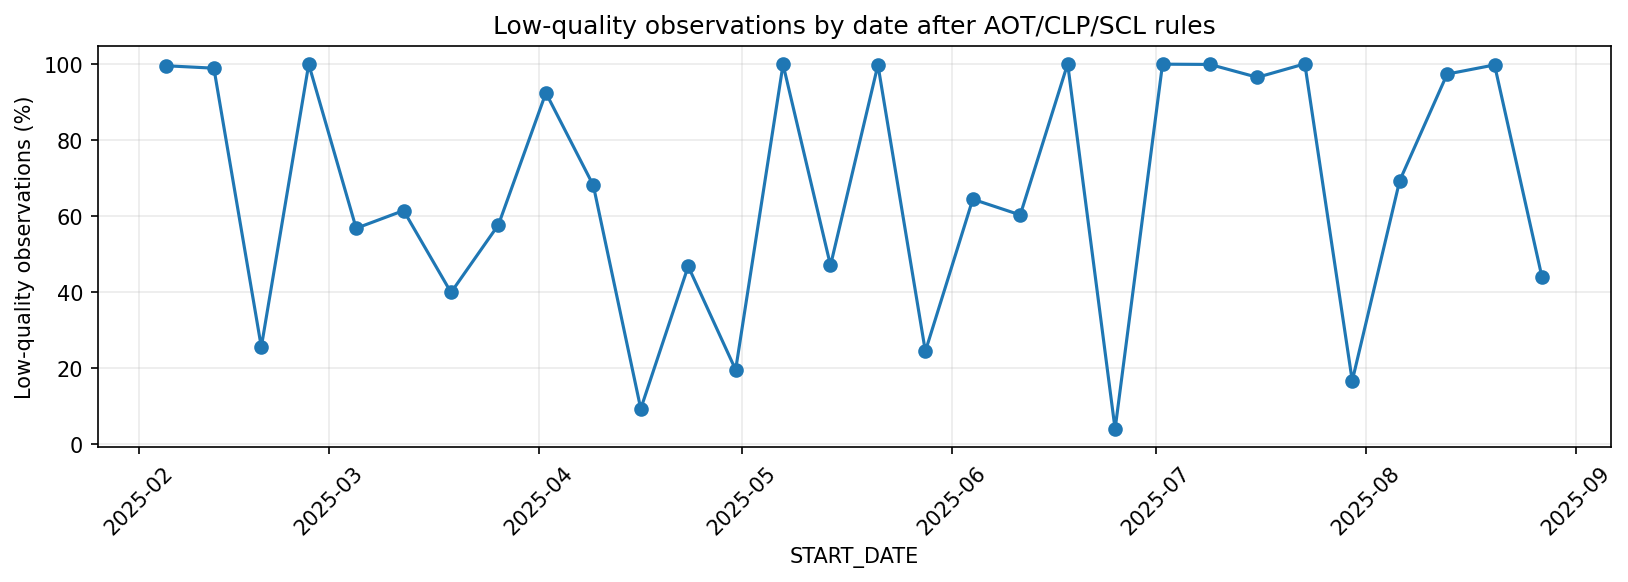
\includegraphics[width=\textwidth]{figures/low_quality_observations_by_date.png}
    \caption{Temporal pattern of nullified observations across Season~B~2025.
    Each data point represents one 7-day acquisition date. Strong temporal
    variability in cloud cover motivates the interpolation step.}
    \label{fig:lq_by_date}
\end{figure}


% ------------------------------------------------------------
\subsection{Boundary Pixel Removal}
\label{subsec:boundary}
% ------------------------------------------------------------

A boundary pixel is a QUADKEY for which the same (\texttt{QUADKEY},
\texttt{START\_DATE}) combination is associated with two or more distinct
\texttt{Landcover} labels on the same date. This arises when a QUADKEY
tile straddles the boundary between two different field polygons — for
example, a tile that partially overlaps a maize field and a bean field
simultaneously. The resulting spectral observation is a mixture of two
crop phenologies and cannot be reliably assigned to either class, so all
such QUADKEYs are removed.

Crucially, boundary pixel removal is performed \emph{before} gap analysis.
Performing it afterwards would risk including conflicting observations in
the gap statistics, inflating the reported maximum gap length with noise
from boundary tiles rather than genuine cloud-induced missingness.
The conflict check identified one such QUADKEY, classified as a
cross-polygon / cross-farm boundary, consistently appearing across all
30 acquisition dates. This QUADKEY was removed.


% ------------------------------------------------------------
\subsection{Temporal Gap Analysis and Linear Interpolation}
\label{subsec:interpolation}
% ------------------------------------------------------------

\subsubsection{Time Cadence Verification}
\label{subsubsec:cadence}

Before gap analysis, the acquisition cadence is verified by computing
pairwise date differences within each QUADKEY's time series. All
consecutive \texttt{START\_DATE} intervals are exactly 7~days, confirming
a perfectly regular weekly grid. A gap of $k$ consecutive nullified
observations therefore corresponds to $k \times 7$~days without valid
spectral data.

\subsubsection{Gap Statistics and QUADKEY Removal}
\label{subsubsec:gap}

For each QUADKEY, the lengths of consecutive null-spectral segments are
computed. The maximum gap length per QUADKEY is used as the criterion for
removal. The maximum allowable gap is set to 9 consecutive missing
observations (equivalent to 63 consecutive days). QUADKEYs whose maximum
gap exceeds this threshold are discarded, because interpolating across a
gap longer than nine observations would generate speculative values that
bear little resemblance to actual spectral dynamics and could introduce
spurious phenological features. Figure~\ref{fig:gap_dist} shows the
distribution of maximum gap lengths across all QUADKEYs.

\begin{figure}[H]
    \centering
    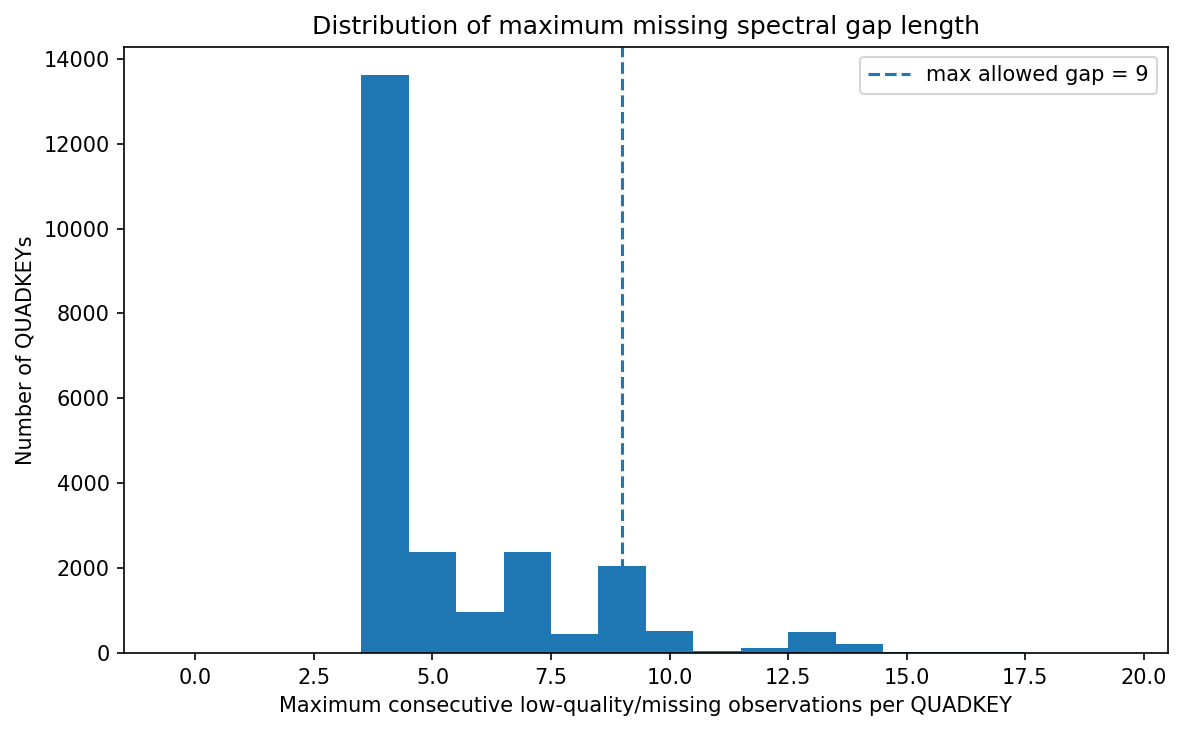
\includegraphics[width=\textwidth]{figures/max_missing_gap_length_distribution.png}
    \caption{Histogram of the maximum consecutive missing observation
    gap per QUADKEY after quality-control nullification. The dashed vertical
    line marks the removal threshold at 9 consecutive missing observations.}
    \label{fig:gap_dist}
\end{figure}

\subsubsection{Linear Interpolation}
\label{subsubsec:linear_interp}

For QUADKEYs whose maximum gap does not exceed the threshold, missing
spectral values are filled using \textbf{linear interpolation} applied
independently to each spectral band column within each QUADKEY's time
series.

Linear interpolation was chosen over more complex alternatives for several
reasons. First, within limited missing gaps, Sentinel-2 vegetation signals
are expected to change gradually because crop development follows a broadly
smooth seasonal trajectory, with green-up, peak canopy development, and
senescence phases. Over such gaps, linear interpolation provides a
reasonable local approximation to the trajectory without requiring
assumptions about the specific functional form of the phenological curve.
Second, more complex methods such as
Savitzky--Golay smoothing or double-logistic fitting require a sufficient
number of valid observations to fit reliably, which is not guaranteed in
heavily cloud-affected time series. Third, linear interpolation is
computationally inexpensive and deterministic, supporting reproducibility.

After interpolation, a temporal coverage check confirms that all remaining
QUADKEYs have exactly 30 valid observations spanning the Season~B window.
The final preprocessed dataset contains 655,950 observations across
21,865 QUADKEYs.


% ============================================================
\section{Feature Engineering}
\label{sec:features}
% ============================================================

Feature engineering transforms the preprocessed time series into a
tabular feature matrix suitable for classical machine learning models,
while also preserving the temporal structure for deep learning. For each
QUADKEY, features are extracted from its 30-observation time series across
15 vegetation indices, yielding a final feature matrix of shape
$21{,}865 \times 96$.


% ------------------------------------------------------------
\subsection{Vegetation Index Computation}
\label{subsec:vi}
% ------------------------------------------------------------

Vegetation indices are computed from the scaled Sentinel-2 reflectance
bands after interpolation. They serve as physically meaningful
transformations of the raw spectral bands, accentuating specific aspects
of vegetation state (greenness, moisture, canopy structure, stress)
that are more directly related to crop type and phenological stage than
individual band values. The complete list of all 15 vegetation indices,
including formulas, Sentinel-2 bands, and agronomic interpretation, is
provided in Appendix~\ref{app:detailed_methodology_tables}
(Table~\ref{tab:vi}).


% ------------------------------------------------------------
\subsection{Statistical Feature Extraction}
\label{subsec:stat_features}
% ------------------------------------------------------------

For each of the 15 vegetation indices, four summary statistics are
computed per QUADKEY over its 30-observation time series:

\begin{equation}
\label{eq:stat_features}
\{\bar{x},\ \sigma,\ x_{\min},\ x_{\max}\}
\end{equation}

where $\bar{x}$ is the temporal mean, $\sigma$ the standard deviation,
$x_{\min}$ the minimum, and $x_{\max}$ the maximum value across the
Season~B window. These statistics capture the central tendency, temporal
variability, and seasonal range of each spectral signal, providing a
compact but informative representation of each QUADKEY's growing season
trajectory. This yields $15 \times 4 = 60$ statistical features per
QUADKEY.


% ------------------------------------------------------------
\subsection{Phenological Feature Extraction}
\label{subsec:pheno_features}
% ------------------------------------------------------------

Six phenological metrics are extracted from the time series of six
selected vegetation indices (NDVI, EVI, NDMI, LSWI, NDRE, NBR) that
exhibit a clear seasonal signal over the crop growth cycle. The
phenological extraction follows the \textbf{TIMESAT left-minimum
approach}~\cite{jonsson2004}: the start of season (SoS) is defined not
as the global minimum of the series, but as the local minimum on the
\emph{left side} of the seasonal peak. This approach avoids the problem
where noisy or cloud-affected observations at the beginning of the time
series cause SoS to default to time step~0.

The six phenological features extracted per index per QUADKEY are:

\begin{enumerate}
    \item \textbf{SoS (Start of Season):} the index of the left-side
          local minimum, representing the onset of green-up. Formally,
          the left series is defined as $x_{1:\hat{t}+1}$ where
          $\hat{t} = \arg\max(x)$, and SoS is the index of the minimum
          within this left segment.
    \item \textbf{EoS (End of Season):} the index at which the right side
          of the seasonal curve falls below the SoS threshold value,
          representing senescence.
    \item \textbf{Peak Value:} $x_{\hat{t}}$, the maximum value of the
          index over the Season~B window.
    \item \textbf{Amplitude:} $x_{\hat{t}} - x_{\mathrm{SoS}}$, the
          seasonal swing of the vegetation index from green-up onset to
          peak.
    \item \textbf{Rate of Increase:} $\dfrac{\mathrm{Amplitude}}{\hat{t} -
          \mathrm{SoS}}$, the average rate of greenness increase per time
          step during the growing phase.
    \item \textbf{Integral:} $\displaystyle\int_{\mathrm{SoS}}^{\mathrm{EoS}}
          x(t)\,dt$, approximated by the trapezoidal rule over the growing
          season segment, representing accumulated photosynthetic activity.
\end{enumerate}

The SoS threshold is computed as:
\begin{equation}
\label{eq:sos_threshold}
\theta_{\mathrm{SoS}} = x_{\mathrm{left\,min}} + 0.20 \times (x_{\hat{t}} - x_{\mathrm{left\,min}})
\end{equation}
encoding that SoS is the point at which the index rises to 20\% of the
seasonal amplitude above the left-side minimum.

With 6 phenological features computed for each of 6 indices, this yields
$6 \times 6 = 36$ phenological features per QUADKEY.


% ------------------------------------------------------------
\subsection{Final Feature Matrix}
\label{subsec:feature_matrix}
% ------------------------------------------------------------

Combining the 60 statistical features (Section~\ref{subsec:stat_features})
and the 36 phenological features (Section~\ref{subsec:pheno_features})
produces a final feature matrix of shape $21{,}865 \times 96$
(21,865~QUADKEYs, 96 features per QUADKEY). No additional dimensionality
reduction is applied at this stage; feature selection is performed as part
of the model development pipeline (Section~\ref{subsec:feat_sel}) using
the training subset only, to prevent information from the test set
influencing feature selection.

The feature matrix is saved to
\texttt{artifacts/monocrop\_model\_features.parquet} and the list of
feature column names to \texttt{artifacts/feature\_columns.json} for
reproducible downstream use.


% ============================================================
\section{Exploratory Data Analysis}
\label{sec:eda}
% ============================================================

Exploratory Data Analysis (EDA) is conducted at two stages of the
pipeline: (1)~after preprocessing and class selection, to characterise
the cleaned dataset, and (2)~after feature engineering, to assess the
discriminative power and inter-feature relationships of the extracted
features. EDA findings directly inform subsequent modelling choices,
including the class imbalance strategy and the feature selection approach.


% ------------------------------------------------------------
\subsection{Univariate Analysis}
\label{subsec:univariate}
% ------------------------------------------------------------

\paragraph{Class distribution.}
Figure~\ref{fig:class_dist} shows the distribution of unique QUADKEYs per
crop class after label standardisation and monocrop filtering, before the
later temporal gap filtering step. MAIZE dominates the dataset with
12,460 QUADKEYs (53.4\%), followed by RICE with 8,679 (37.2\%),
IRISH POTATO with 1,161 (5.0\%), and BEAN with 1,040 (4.5\%). This
severe class imbalance motivates the use of a resampling strategy during
model training (Section~\ref{subsec:class_imbalance}).

\begin{figure}[H]
    \centering
    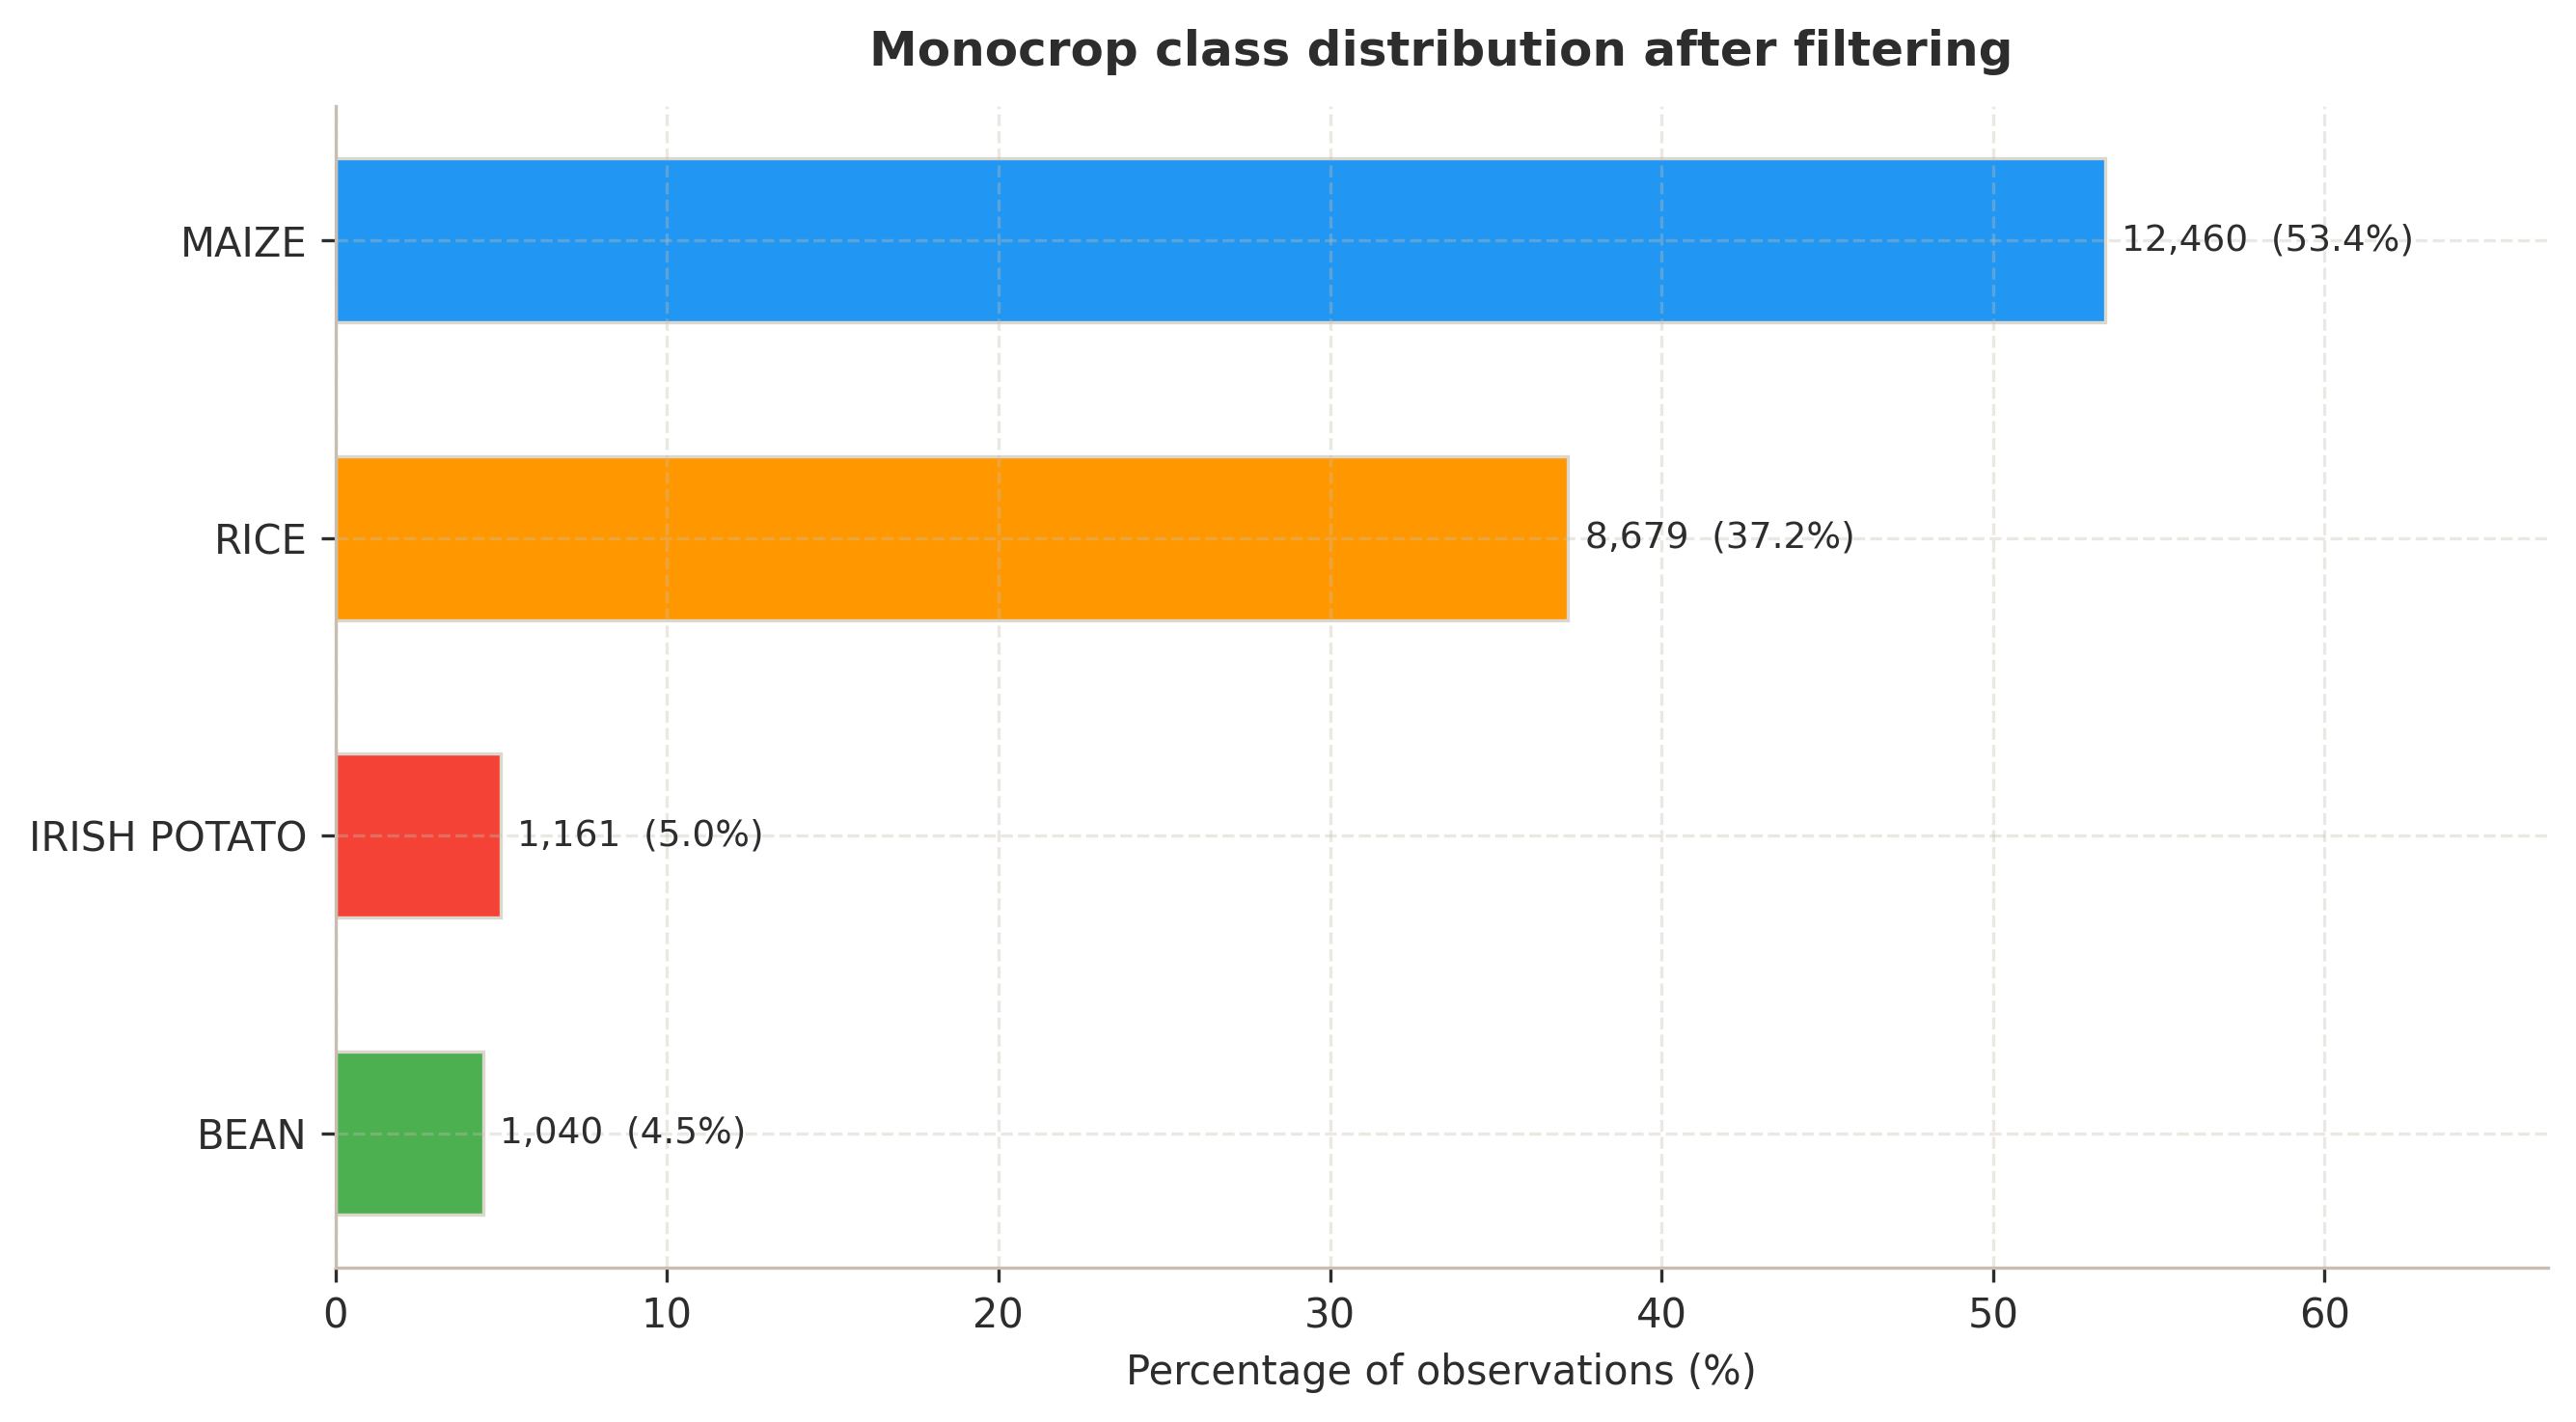
\includegraphics[width=\textwidth]{figures/crop_distribution_monocrop.png}
    \caption{Distribution of unique QUADKEYs per monocrop class after
    filtering. MAIZE and RICE dominate the dataset, while IRISH POTATO
    and BEAN form much smaller minority classes.}
    \label{fig:class_dist}
\end{figure}

\paragraph{Per-class vegetation index box plots.}
Box plots of key vegetation indices stratified by crop class
(Figure~\ref{fig:boxplots}) provide a first visual assessment of
inter-class discriminability. Indices that show minimal overlap between
class distributions are candidates for strong predictors in the
classification model.

\begin{figure}[H]
    \centering
    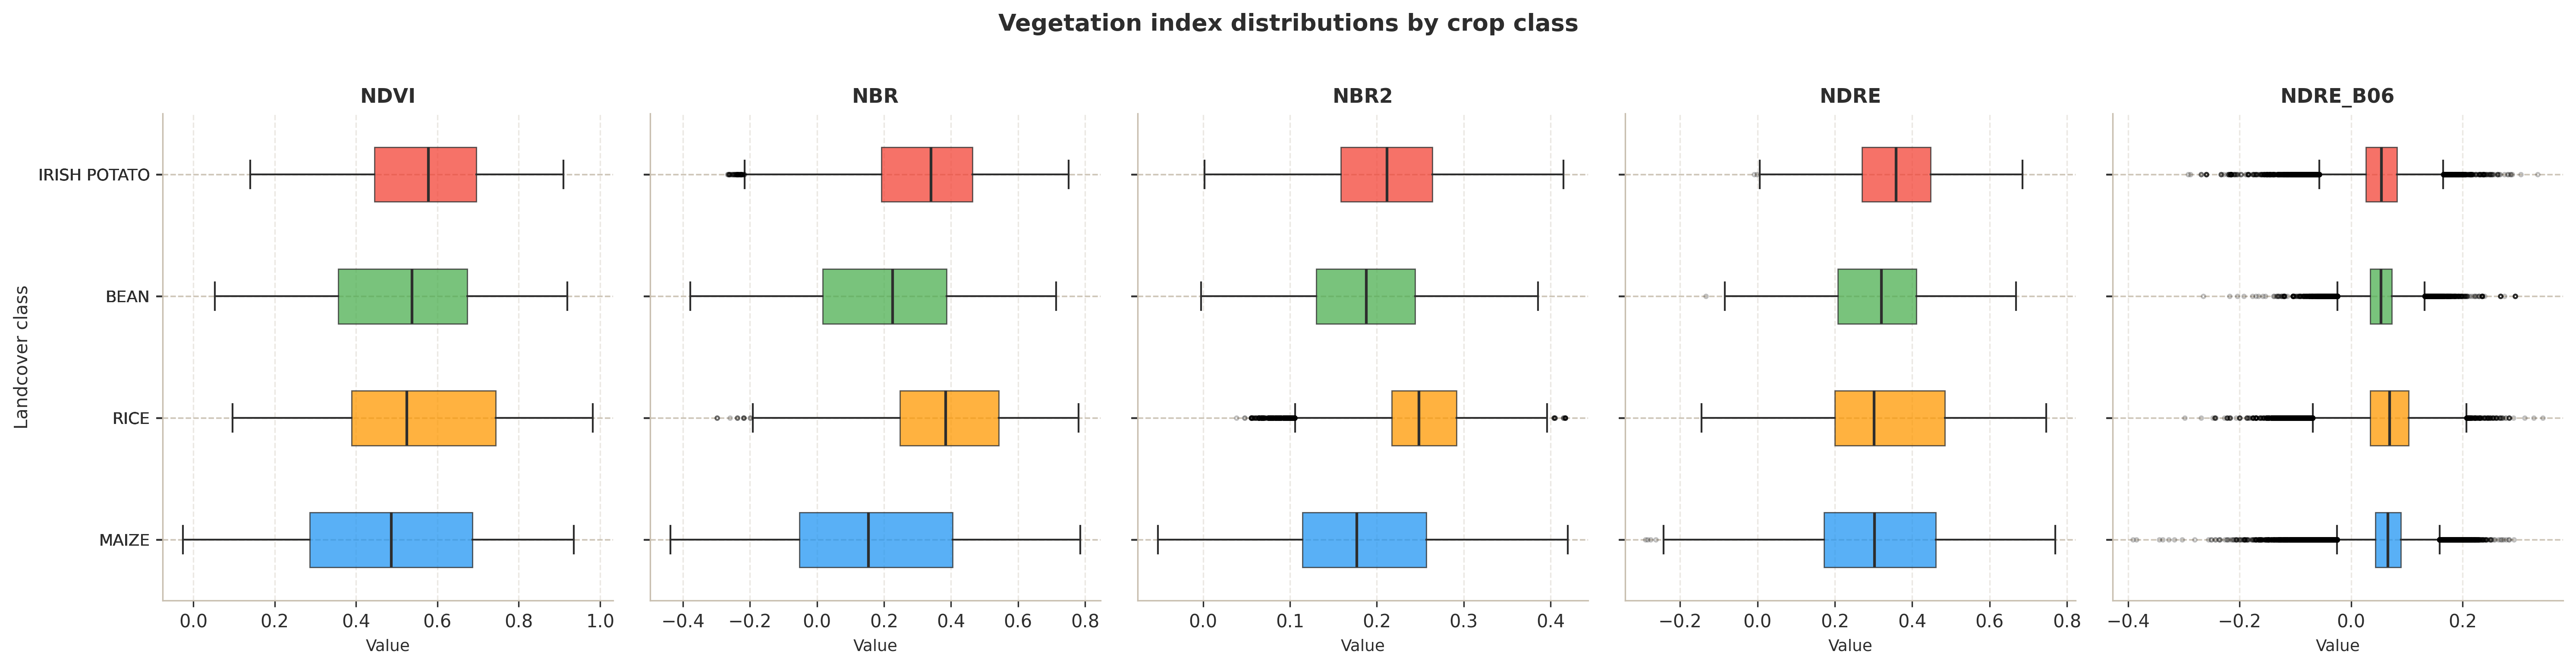
\includegraphics[width=\textwidth]{figures/vi_boxplots_grouped.png}
    \caption{Box plots of key vegetation index values by crop class.
    Overlapping interquartile ranges indicate class separation difficulty;
    non-overlapping ranges suggest strong discriminative features.}
    \label{fig:boxplots}
\end{figure}


% ------------------------------------------------------------
\subsection{Bivariate Analysis}
\label{subsec:bivariate}
% ------------------------------------------------------------

\paragraph{Feature correlation heatmap.}
A Pearson correlation heatmap is computed for the selected engineered
features (Figure~\ref{fig:corr_heatmap}). Several feature pairs exhibit
near-perfect correlation: NDMI and LSWI share a correlation of 1.000,
as they use an identical formula under the Sentinel-2 band configuration;
NDMI and NBR have a correlation of 0.991; and NDRE and CI\_RE have a
correlation of 0.949. These high correlations motivate the three-stage
feature selection procedure (Section~\ref{subsec:feat_sel}), which removes
redundant features before model training.

\paragraph{Temporal crop signatures.}
Mean vegetation index time series are plotted per crop class across the
30-observation Season~B window to visualise class-specific phenological
patterns (Figure~\ref{fig:temporal_sigs}). Differences in peak timing,
amplitude, and green-up rate between classes provide qualitative
justification for including phenological features in the model.

\begin{figure}[H]
    \centering
    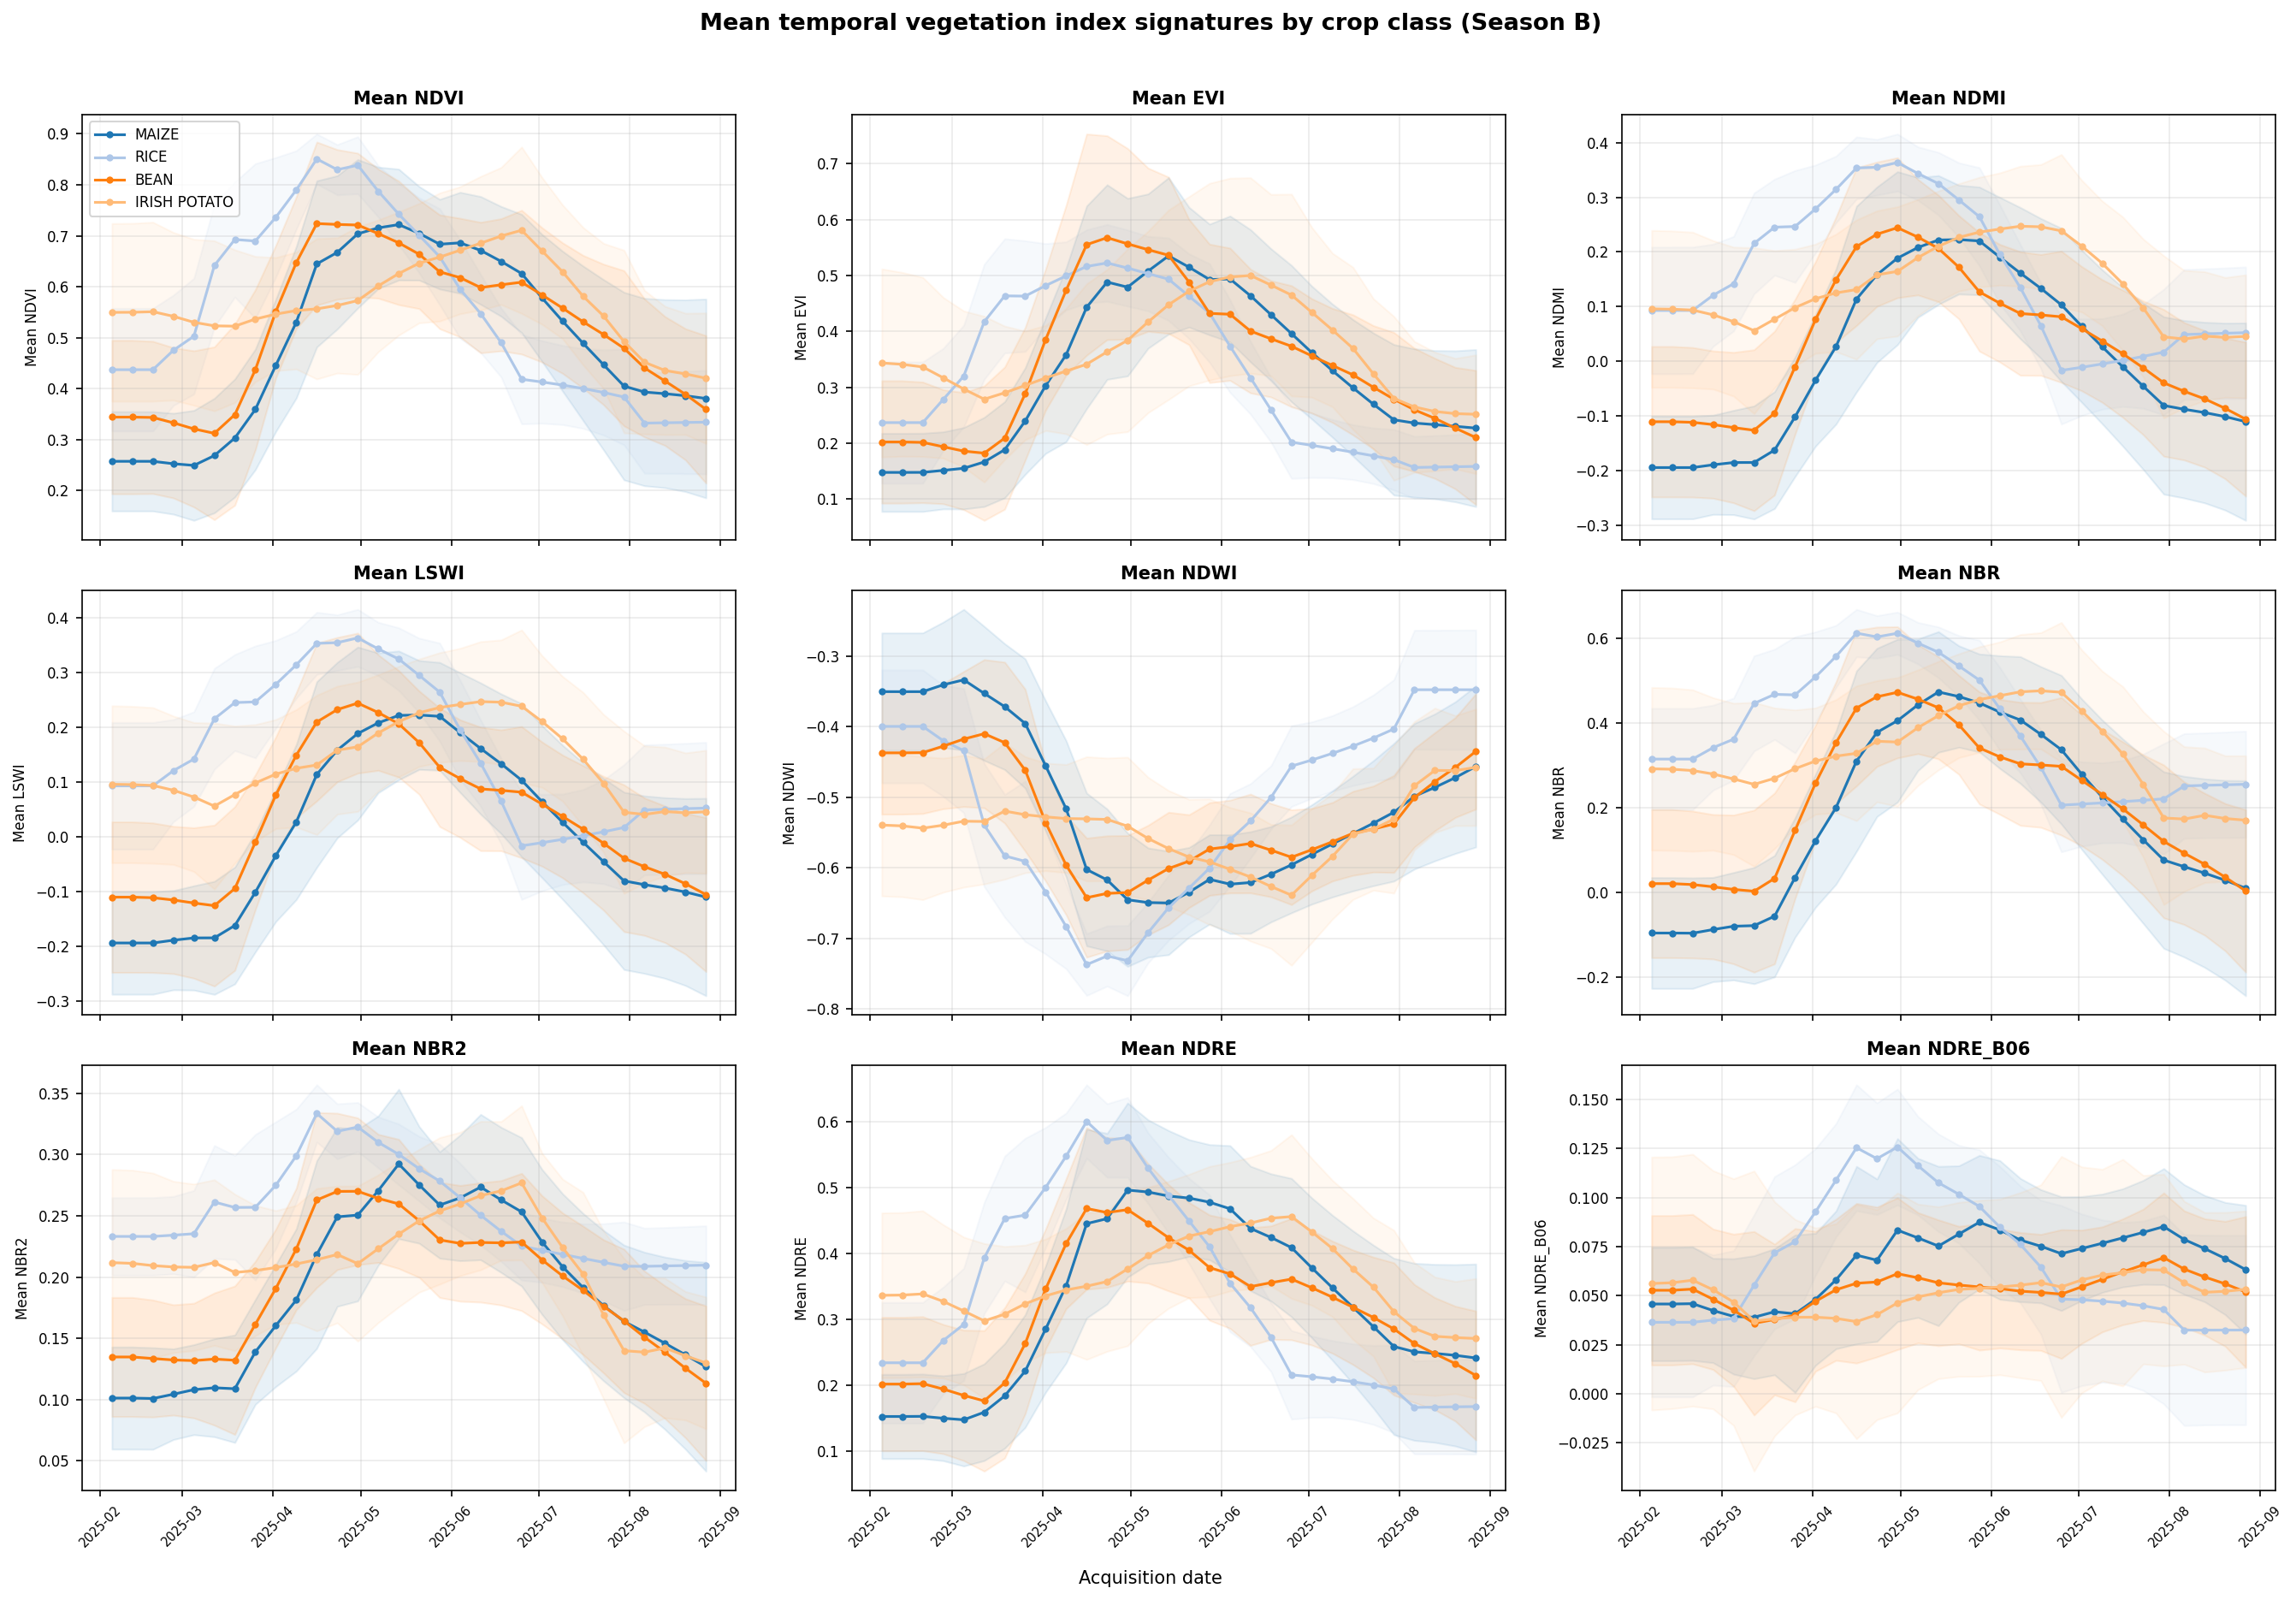
\includegraphics[width=\textwidth]{figures/temporal_crop_signatures_grouped.png}
    \caption{Mean temporal profiles of key vegetation indices per crop
    class across Season~B~2025. Class-specific differences in phenological
    timing and magnitude underpin the feature engineering choices.}
    \label{fig:temporal_sigs}
\end{figure}


% ------------------------------------------------------------
\subsection{Multivariate Analysis}
\label{subsec:multivariate}
% ------------------------------------------------------------

\paragraph{Within-class consistency.}
A well-labelled crop class should be spectrally similar across all its
pixels. If pixels labelled as \textit{Maize} look very different from one
another in the satellite data, the classifier will struggle to learn a
reliable decision boundary for that class. Two metrics are used to quantify
this internal consistency for each class, computed across four vegetation
indices (NDVI, EVI, NDMI, NDRE):

\begin{itemize}
    \item \textbf{Within-date standard deviation:} on each acquisition date,
          the standard deviation of the index value is computed across all
          QUADKEYs belonging to the same class. A high value means that on
          any given day, pixels of the same crop type look spectrally very
          different from each other — indicating a heterogeneous class.

    \item \textbf{Quadkey mean standard deviation:} for each QUADKEY, the
          seasonal mean of the index is computed across all 30 dates. The
          standard deviation of these seasonal means across all QUADKEYs
          of the same class is then taken. A high value means that different
          pixels of the same crop follow very different seasonal trajectories
          — some growing fast, others slowly — making the class harder to
          characterise with a single phenological profile.
\end{itemize}

Figure~\ref{fig:within_class} presents both metrics for all four classes.
RICE emerges as the most internally consistent class across all indices,
meaning its pixels tend to look similar to each other both at any given
date and across the full season. BEAN and IRISH POTATO show the highest
intra-class variability on both metrics, which partly explains the
classification difficulty evidenced in the PCA separability check
(Figure~\ref{fig:pca}) and motivates the use of expressive non-linear
classifiers.

\begin{figure}[H]
    \centering
    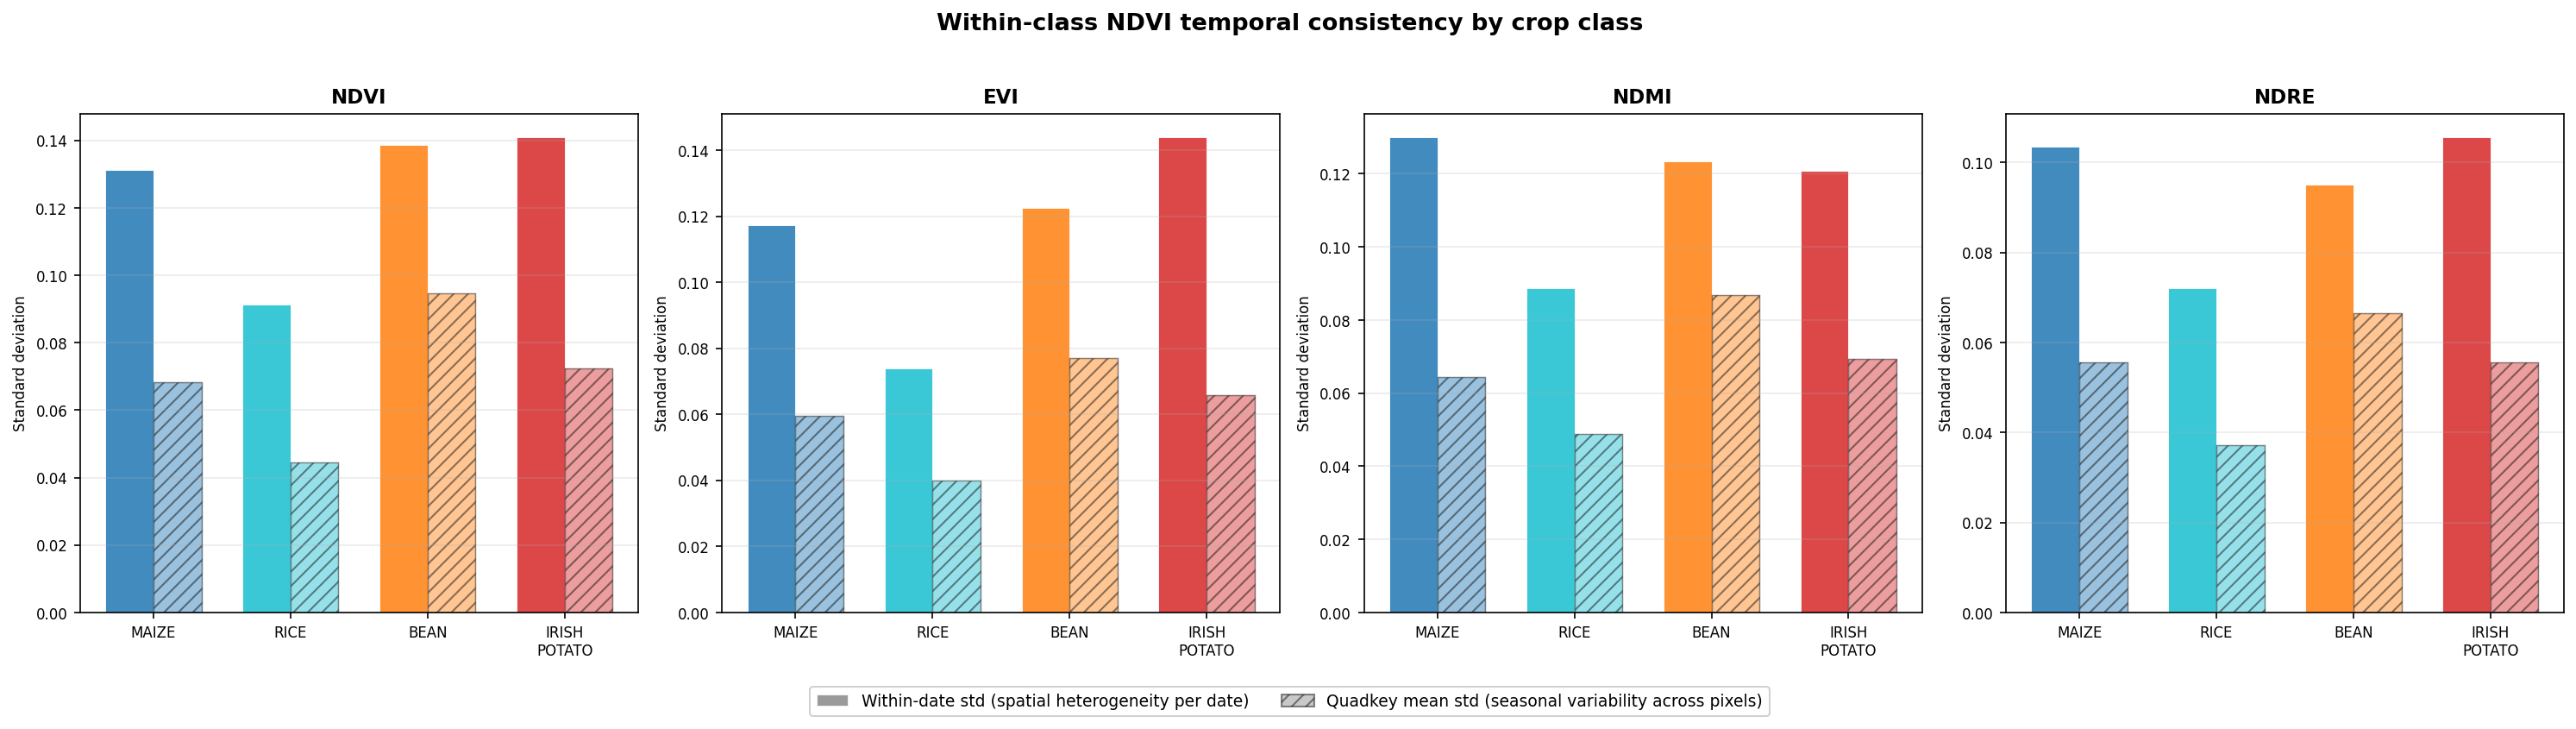
\includegraphics[width=\textwidth]{figures/within_class_consistency.png}
    \caption{Within-class temporal consistency for NDVI, EVI, NDMI, and
    NDRE. Solid bars show within-date standard deviation; hatched bars
    show quadkey mean standard deviation. RICE is the most compact class;
    BEAN and IRISH POTATO show the highest intra-class variability.}
    \label{fig:within_class}
\end{figure}

\paragraph{PCA separability check.}
A Principal Component Analysis (PCA) applied to the mean vegetation-index
feature space provides a two-dimensional visualisation of class
separability (Figure~\ref{fig:pca}). PC1 explains 71.4\% of total
variance and PC2 a further 13.3\%. The PCA plot reveals that RICE and
IRISH POTATO show partial separation along the PC2 axis: RICE clusters
towards negative PC2 values while IRISH POTATO occupies a broader spread
towards positive PC1. MAIZE and BEAN, however, overlap substantially with
each other and with the other classes across both principal components,
confirming that the two-dimensional vegetation-index feature space does
not provide sufficient linear separability. This motivates the use of the
full 96-feature engineered representation and non-linear ensemble
classifiers rather than linear methods.

\begin{figure}[H]
    \centering
    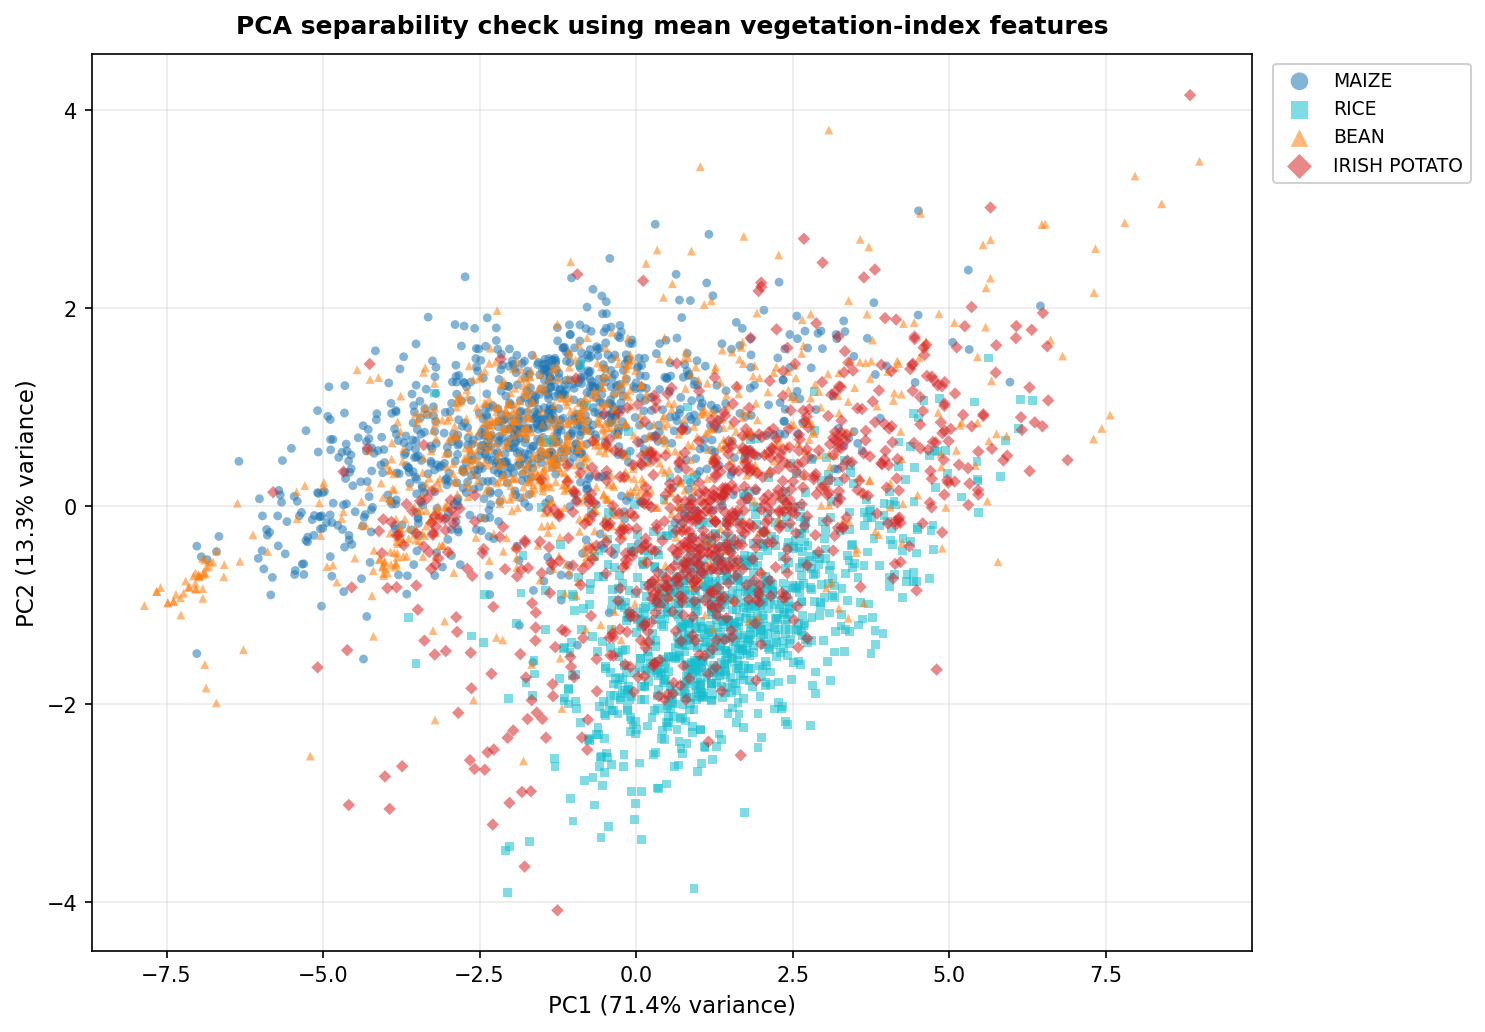
\includegraphics[width=\textwidth]{figures/pca_separability_check.png}
    \caption{Two-dimensional PCA projection of per-QUADKEY mean
    vegetation-index features, coloured and shaped by crop class
    (MAIZE: blue circle; RICE: teal square; BEAN: orange triangle;
    IRISH POTATO: red diamond). PC1 captures 71.4\% of total variance
    and PC2 a further 13.3\%. RICE and IRISH POTATO show partial
    separation along PC2, while MAIZE and BEAN overlap strongly across
    both axes, confirming that linear separation is insufficient.}
    \label{fig:pca}
\end{figure}

\paragraph{Spatial distribution.}
A spatial scatter plot of QUADKEY centroids coloured by crop class
(Figure~\ref{fig:spatial}) reveals that crop classes are geographically
clustered rather than randomly mixed, consistent with the four-district
collection design. This spatial clustering has implications for how the
train/test split is constructed, as discussed in
Section~\ref{subsec:train_test_split_strategy}.

\begin{figure}[H]
    \centering
    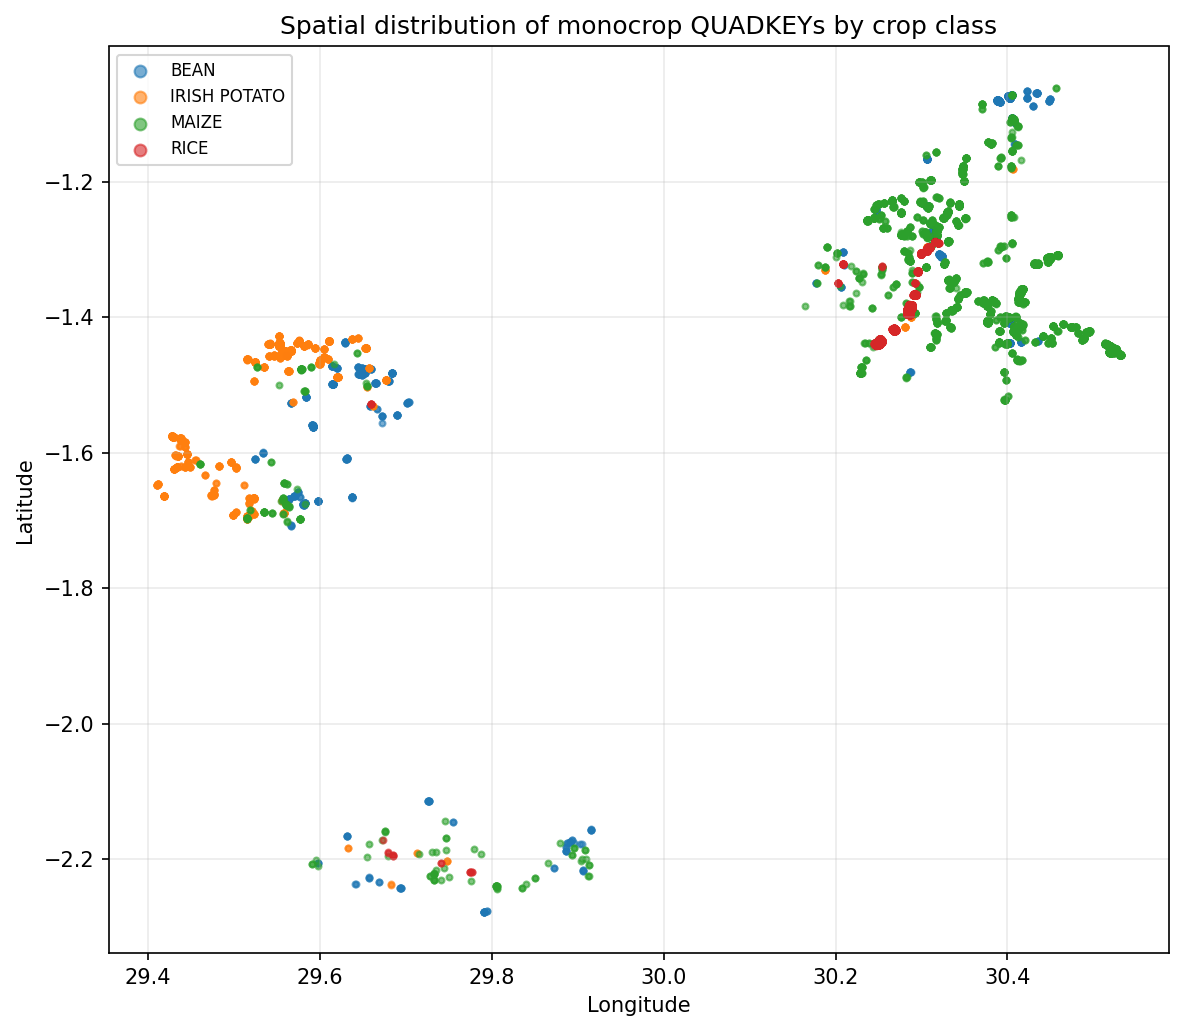
\includegraphics[width=\textwidth]{figures/spatial_distribution_monocrop_quadkeys.png}
    \caption{Geographic distribution of QUADKEY centroids coloured by
    crop class across the four surveyed districts of Rwanda. Crop classes
    are geographically clustered, consistent with the district-level
    collection design.}
    \label{fig:spatial}
\end{figure}


% ============================================================
\section{Model Development}
\label{sec:model_dev}
% ============================================================

% ------------------------------------------------------------
\subsection{Train--Test Split Strategy}
\label{subsec:train_test_split_strategy}

Two train--test split strategies were used in this study. The first defines
the main modelling protocol, while the second acts as a spatial robustness
check.

\paragraph{Primary QUADKEY-level split.}
The main experiment uses a stratified QUADKEY-level split. Individual
QUADKEYs are randomly assigned to the training and test partitions using an
80/20 split, with stratification by the \texttt{Landcover} label. This keeps
the crop-class proportions approximately consistent in both partitions, which
is important because the dataset is class-imbalanced.

The training partition is used for feature selection, model comparison,
imbalance-strategy selection, and hyperparameter tuning through internal
cross-validation. The test partition is kept separate as the final test
set. This prevents the test data from influencing model-development
decisions.

\paragraph{Limitation of the QUADKEY-level split.}
The QUADKEY-level split ensures that the exact same QUADKEY does not appear
in both training and test data. However, it does not fully remove the risk of
spatial leakage. Neighbouring QUADKEYs from the same field or polygon may
still be assigned to different partitions.

These neighbouring samples are not fully independent. They may share the same
crop label, soil conditions, field management, planting date, irrigation
regime, local weather exposure, Sentinel-2 acquisition conditions, and
annotation source. Therefore, a model evaluated on neighbouring tiles from a
field already represented in training may appear to generalise better than it
would on entirely unseen fields.

\paragraph{Field-level group-aware split.}
To assess this risk, a second split was created as a spatial leakage
robustness check. This split uses \texttt{StratifiedGroupKFold} with five
folds. The grouping variable is the field or polygon identifier \texttt{id},
which links each QUADKEY to its source ground-truth polygon.

All QUADKEYs belonging to the same field or polygon group are kept in the
same partition. Therefore, no field group appears in both the training and
test sets. The first fold is used as the test fold, giving an
approximately 80/20 group-aware split.

\paragraph{Use of the field identifier.}
The field identifier is used only for grouping and leakage diagnosis. It is
not used as a model input feature. Including \texttt{id} as a predictor would
make the experiment unrealistic because it is not an Earth-observation crop
signal and would not be available for unseen fields during operational
inference.

\paragraph{Stratification.}
Stratification by \texttt{Landcover} is applied in both split protocols. In
the QUADKEY-level split, stratification preserves class proportions across
individual QUADKEY samples. In the group-aware split, stratification is
applied while respecting field boundaries, so class balance is preserved as
much as possible without allowing samples from the same field or polygon to
appear in both partitions.


% ------------------------------------------------------------
\subsection{Feature Selection}
\label{subsec:feat_sel}
% ------------------------------------------------------------

Feature selection is applied \emph{exclusively on the training set},
before any resampling, to ensure that the selection process is not
influenced by synthetic samples or by the test set. A three-stage
selection pipeline is employed:

\begin{enumerate}
    \item \textbf{Stage 1 — ANOVA $F$-test:} A one-way analysis of variance
          $F$-test (\texttt{f\_oneway} from \texttt{scipy.stats}) is applied
          to each of the 96 features independently on the training set,
          testing for differences in feature means across the four crop
          classes. To control the family-wise error rate across all 96
          simultaneous tests, a \textbf{Bonferroni correction} is applied:
          the significance threshold is set to
          $\alpha_{\mathrm{Bonferroni}} = \alpha / n_{\mathrm{features}} = 0.05 / 96$.
          Only features whose $p$-value falls below this corrected threshold
          are retained for the next stage.

    \item \textbf{Stage 2 — Random Forest Importance:} A Random
          Forest~\cite{breiman2001randomforest} classifier is trained on
          the training set and feature importances (mean decrease in
          impurity) are computed and ranked. The
          top-$k$ features by importance are retained for the next stage.

    \item \textbf{Stage 3 — Recursive Feature Elimination (RFE):} RFE
          with 5-fold cross-validation (\texttt{RFECV}) iteratively removes
          the least important features, selecting the subset that maximises
          cross-validated macro F1. The final selected feature set is saved
          to \texttt{artifacts/selected\_features.json}.
\end{enumerate}

This cascaded approach progressively removes redundant and non-discriminative
features, reducing model complexity and training time while retaining the
features most relevant to crop classification.


% ------------------------------------------------------------
\subsection{Class Imbalance Handling}
\label{subsec:class_imbalance}
% ------------------------------------------------------------

The monocrop training set is strongly imbalanced. In the QUADKEY-level
training partition, the class distribution is dominated by MAIZE and RICE,
while BEAN and IRISH POTATO are much less frequent:

\[
\text{MAIZE}=9{,}843,\quad
\text{RICE}=6{,}194,\quad
\text{BEAN}=814,\quad
\text{IRISH POTATO}=641.
\]

Thus, MAIZE and RICE together account for approximately \(91.7\%\) of the
training samples, while BEAN and IRISH POTATO together account for only
approximately \(8.3\%\). This imbalance is important because a classifier
trained directly on the original distribution may favour the majority
classes and still obtain high overall accuracy, while performing poorly on
minority crops. For this reason, class imbalance was addressed explicitly
during model development using cost-sensitive learning and synthetic
minority oversampling.

\paragraph{Compared imbalance strategies.}
Three families of imbalance strategies were evaluated: balanced class
weights, synthetic minority oversampling using SMOTE~\cite{chawla2002smote},
and Adaptive Synthetic Sampling (ADASYN)~\cite{he2008adasyn}. Class
weights increase the penalty assigned to mistakes on minority crops without
changing the training distribution. SMOTE and ADASYN instead alter the
training distribution by generating additional minority-class examples.
All resampling was performed strictly inside each cross-validation fold to
avoid validation leakage. The detailed weighting equations, SMOTE and
ADASYN formulas, target counts, and leakage-safe resampling diagram are
given in Appendix~\ref{app:model_evaluation_details}.

\paragraph{Final imbalance strategy selection by average rank across top models.}
The imbalance strategies were compared using stratified 5-fold
cross-validation on the training data, evaluated \emph{independently for
each of the three top-benchmark models} identified in
Section~\ref{subsec:benchmarking}. For each model, each strategy is
ranked by its mean cross-validated macro F1. The final strategy is
selected by \textbf{average rank across the three models}: the strategy
with the lowest average rank (i.e., most consistently strong across all
three model families) is chosen. This cross-model selection criterion
avoids choosing a strategy that is only well-suited to one model family.

Figure~\ref{fig:imbalance_comparison} summarises the cross-validated macro
F1 for all tested strategies. The \textbf{per-class SMOTE medium} strategy
achieved an average rank of 1.67 across the three top models, the lowest
of all candidates, making it the selected strategy for the final pipeline.
It oversamples BEAN and IRISH POTATO to approximately \(60\%\) of the
RICE training count, providing a moderate compromise between leaving the
minority classes under-represented and generating an excessive number of
synthetic samples.

\paragraph{Deep learning sequence training.}
For the sequence-based LSTM, GRU, and 1D CNN models, SMOTE and ADASYN were
not applied because the models operate on temporal sequence tensors rather
than fixed-length tabular features. Class imbalance was therefore handled
using balanced class weights passed to the Keras \texttt{fit()} method.
The corresponding weighted loss expression is provided in
Appendix~\ref{app:model_evaluation_details}.


% ------------------------------------------------------------
\subsection{Machine Learning Models}
\label{subsec:benchmarking}
% ------------------------------------------------------------

Five classical machine learning classifiers are benchmarked using
5-fold stratified cross-validation on the training set:

\begin{enumerate}
    \item \textbf{Random Forest}~\cite{breiman2001randomforest}
          (\texttt{n\_estimators = 250},
          \texttt{class\_weight = "balanced"});
    \item \textbf{Extra Trees}~\cite{geurts2006extratrees}
          (\texttt{n\_estimators = 300},
          \texttt{class\_weight = "balanced"});
    \item \textbf{XGBoost}~\cite{chen2016xgboost}
          (\texttt{n\_estimators = 300},
          \texttt{max\_depth = 5},
          \texttt{learning\_rate = 0.05},
          \texttt{objective = "multi:softprob"});
    \item \textbf{Gradient Boosting} (sklearn implementation, with
          sample weighting);
    \item \textbf{Linear SVM} (scaled features,
          \texttt{class\_weight = "balanced"}).
\end{enumerate}

All models are evaluated using macro F1 as the primary metric, which
equally weights all four classes regardless of their support size.
Additional metrics recorded per fold include weighted F1, balanced
accuracy, Cohen's kappa~\cite{cohen1960kappa}, and geometric mean
(G-mean) of per-class recalls. The test set remains entirely
untouched during this benchmarking phase.

\paragraph{Top-3 model selection.}
After benchmarking, the three models with the highest mean cross-validated
macro F1 are selected for the subsequent imbalance strategy comparison and
hyperparameter tuning stages. This approach avoids committing to a single
model before the imbalance strategy has been determined, since the optimal
strategy may vary across model families. The selected top-3 model names
and their cross-validation scores are saved to
\texttt{artifacts/top3\_benchmark\_models.json} and
\texttt{artifacts/best\_benchmark\_model.json} respectively, forming the
sole basis on which the downstream notebooks identify which models to tune.
The test set is not consulted at this stage.


% ------------------------------------------------------------
\subsection{Hyperparameter Tuning}
\label{subsec:tuning}
% ------------------------------------------------------------

Hyperparameter tuning is applied to \emph{all three top-benchmark models}
identified in Section~\ref{subsec:benchmarking} (Extra Trees, XGBoost,
and Random Forest), using the per-class SMOTE medium imbalance strategy
selected in Section~\ref{subsec:class_imbalance}. Each model is tuned
independently using \textbf{Randomised Search Cross-Validation}
(\texttt{RandomizedSearchCV}) with 5-fold stratified cross-validation
and 20 candidate parameter combinations drawn randomly from the search
spaces reported in Appendix~\ref{app:model_evaluation_details}
(Table~\ref{tab:search_spaces}), totalling 100 fits per model. Tuning is
conducted on the training set only; the test set remains unused until the
final evaluation.

The model with the highest cross-validated macro F1 after tuning is
designated the \textbf{best tuned model} and used for all subsequent
final evaluation, per-class threshold calibration, and district-scale
inference. The resulting benchmark defaults and tuned configurations for
all five models are documented in Appendix~\ref{app:model_evaluation_details}
(Table~\ref{tab:hyperparams}).

% ------------------------------------------------------------
\subsection{Deep Learning Sequence Models}
\label{subsec:deep_learning}
% ------------------------------------------------------------

In addition to classical feature-based models, three deep learning
sequence architectures are evaluated directly on the Sentinel-2 time
series, without the feature engineering step. This allows a direct
comparison between hand-crafted feature representations and learned
temporal representations, and assesses whether the sequential structure
of the 30-observation time series carries discriminative information
beyond what the statistical and phenological features capture.

Each QUADKEY's 30-observation sequence of spectral and index values is
treated as the input tensor of shape $(30, F)$, where $F$ is the number
of sequence feature channels. Three architectures are evaluated:

\begin{enumerate}
    \item \textbf{LSTM (Long Short-Term Memory)~\cite{hochreiter1997}:}
          LSTM is a recurrent neural network architecture designed to model
          temporal dependencies in sequential data. It uses input, forget,
          and output gates to control how information is stored, updated, and
          passed forward through time. This makes it suitable for crop
          phenology, where early-season spectral behaviour may influence
          later-season crop development.

    \item \textbf{GRU (Gated Recurrent Unit)~\cite{cho2014}:}
          GRU is another recurrent architecture for sequence modelling. It is
          simpler than LSTM because it uses fewer gates, mainly update and
          reset gates. This reduces the number of trainable parameters while
          still allowing the model to retain useful temporal information. GRU
          is therefore useful as a lighter recurrent alternative to LSTM for
          the 30-date Sentinel-2 crop sequence.

    \item \textbf{1D CNN (One-Dimensional Convolutional Neural Network):}
          The 1D CNN model treats the Sentinel-2 time series as a temporal
          signal and applies convolutional filters along the time dimension.
          These filters can learn local temporal patterns, such as rapid
          green-up, short-term moisture change, or senescence-related
          decreases in vegetation indices. Unlike recurrent models, the 1D
          CNN does not process the sequence step by step; instead, it learns
          temporal filters in parallel, making it computationally efficient.
\end{enumerate}

The detailed layer diagrams for the LSTM, GRU, and 1D CNN architectures
are provided in Appendix~\ref{app:model_evaluation_details}
(Figures~\ref{fig:lstm_arch}--\ref{fig:cnn_arch}).

All three deep learning models use the same sequence dataset and the same
train/test partition as the classical models. Only QUADKEYs with complete
30-date sequences are included, ensuring a uniform input shape across all
sequence models. Before training, the sequence features are standardised
using the mean and standard deviation computed from the training partition
only, preventing information from the test set from entering the
preprocessing step.

The models are trained for a maximum of 75 epochs with a batch size of 128.
Early stopping monitors the validation loss with a patience of eight epochs
and restores the best validation-loss weights. Class imbalance is handled
through class weights computed from the training labels and passed to the
Keras \texttt{fit()} method. SMOTE and ADASYN are not applied to the sequence
models because these methods are designed for fixed-length tabular feature
vectors, whereas the deep learning models operate on temporal sequence
tensors. Applying synthetic interpolation directly to crop time series could
produce artificial temporal profiles that do not correspond to realistic crop
phenology.


% ============================================================
\section{Per-Class Confidence Threshold Calibration}
\label{sec:thresholds}
% ============================================================

Following final model selection, class-specific confidence thresholds are
calibrated on the test set. Standard classifier output assigns
each QUADKEY the class with the highest predicted probability, regardless
of whether that probability is high or low. In a four-class imbalanced
setting, this can lead to low-confidence predictions for minority classes
being silently accepted. Per-class thresholding addresses this by requiring
the predicted probability for a class to exceed a class-specific minimum
before the label is confirmed.

For each class $c$, the optimal threshold $\tau_c$ is found by a grid
search over candidate values in the range $[0.05, 0.95]$ at a step of
$0.0025$. For each candidate threshold, the per-class F1 score is
computed on the test set by applying the rule:

\begin{equation}
\hat{y}_i =
\begin{cases}
c & \text{if } \hat{p}_{i,c} \geq \tau_c \\
\texttt{uncertain} & \text{otherwise}
\end{cases}
\end{equation}

where $\hat{p}_{i,c}$ is the predicted probability of the argmax class
$c$ for observation $i$. The threshold that maximises the F1 score for
class $c$ on the test set is selected as $\tau_c$.

The resulting calibrated thresholds are saved to
\texttt{artifacts/per\_class\_thresholds.json} and loaded by the
district-scale inference pipeline. Using the test set for threshold
calibration is acceptable here because the thresholds are not used to
select the model (model selection was completed in
Section~\ref{subsec:tuning} using training-set cross-validation only);
the test set is used solely to calibrate the decision boundary of the
already-chosen model.


% ============================================================
\section{District-Scale Inference}
\label{sec:inference}
% ============================================================

Following model training and evaluation, the final model is applied to
the full Nyagatare district to produce a district-scale crop type map.
Nyagatare was selected as the inference target because it is both the
most agriculturally active district in the Harvard Dataverse collection
and the district with the largest spatial extent of cropland, providing
the most geographically meaningful demonstration of the pipeline's
operational capacity.

The inference pipeline mirrors the training preprocessing chain exactly,
applying all the same steps in the same order to ensure that the feature
space presented to the model at inference time is consistent with the
feature space used during training.


% ------------------------------------------------------------
\subsection{Inference Preprocessing}
\label{subsec:inference_preprocessing}
% ------------------------------------------------------------

The Nyagatare Sentinel-2 time series is loaded and processed through the
same sequential steps applied during training: temporal filtering to
Season~B~2025 (February--August), full-row deduplication, zero-band row
removal, band scaling, temporal deduplication to the best observation per
ISO week, spectral quality nullification (SCL, AOT, CLP), gap analysis
with linear interpolation, and vegetation index computation. The same
quality-control thresholds (\texttt{GOOD\_SCL = (4, 5)},
\texttt{AOT\_THRESH = 0.3}, \texttt{CLP\_THRESH = 0.4},
\texttt{MAX\_GAP\_OBS = 9}) and the same gap removal criterion are applied.
Statistical and phenological features are then extracted using the same
functions as in training, producing a feature matrix of shape
$N_{\mathrm{infer}} \times 99$ prior to feature subsetting.


% ------------------------------------------------------------
\subsection{Dynamic World Cropland Mask}
\label{subsec:dw_mask}
% ------------------------------------------------------------

Before inference, a \textbf{Dynamic World cropland mask} is applied to
restrict predictions to pixels that are consistently classified as crops
during the Season~B~2025 period. The mask is derived from the Google
Earth Engine Dynamic World V1 product
(\texttt{GOOGLE/DYNAMICWORLD/V1})~\cite{brown2022dynamic}, which provides
a 10-metre land cover classification at high temporal frequency.

The mask is computed using the following steps:
\begin{enumerate}
    \item Filter the Dynamic World image collection to the Nyagatare
          district boundary and the Season~B date range
          (2025-02-01 to 2025-08-31).
    \item Compute the mode land cover label across all available images
          within this window (temporal majority vote).
    \item Retain only pixels where the mode label equals class~4
          (\textit{Crops}) in the Dynamic World classification.
\end{enumerate}
The resulting binary raster is exported from GEE as a GeoTIFF and loaded
into the inference pipeline. QUADKEYs whose centroid falls outside the
cropland mask are excluded from the feature matrix and receive no
prediction. This step reduces the inference population from
$\sim$19.9~million raw QUADKEYs to 4,088,243 cropland QUADKEYs.


% ------------------------------------------------------------
\subsection{Feature Alignment and Inference}
\label{subsec:inference_predict}
% ------------------------------------------------------------

The feature matrix of the 4,088,243 cropland QUADKEYs is subset to the
37 features identified during training-set feature selection
(\texttt{artifacts/selected\_features.json}). Any remaining \texttt{NaN}
values in the inference matrix are imputed with the column-wise median of
the inference set. The feature matrix is then converted to \texttt{float64}
and passed to the trained model's \texttt{predict} and
\texttt{predict\_proba} methods.


% ------------------------------------------------------------
\subsection{Per-Class Thresholding at Inference}
\label{subsec:inference_threshold}
% ------------------------------------------------------------

Predicted class labels are finalised by applying the per-class confidence
thresholds calibrated in Section~\ref{sec:thresholds}. For each QUADKEY,
the model's argmax class $c$ is accepted only if the corresponding class
probability $\hat{p}_{i,c}$ meets or exceeds the threshold $\tau_c$
loaded from \texttt{artifacts/per\_class\_thresholds.json}. If the
probability falls below the threshold, the QUADKEY is assigned the label
\texttt{uncertain}. This mechanism prevents low-confidence predictions
from being silently included in the crop map, and allows the proportion
of uncertain predictions to be reported transparently as a map quality
indicator.


% ============================================================
\section{Evaluation Framework}
\label{sec:evaluation}
% ============================================================

All models are evaluated on test data that are never used during training,
feature selection, imbalance-strategy selection, or hyperparameter tuning.
Two evaluation protocols are reported, as described in
Section~\ref{subsec:train_test_split_strategy}: the QUADKEY-level split as
the primary evaluation protocol, and the field/group-level split as a
secondary spatial leakage robustness check.

The primary metric is macro F1 because it gives equal importance to all
crop classes and therefore reflects minority-class performance more
directly than overall accuracy. Additional metrics include weighted F1,
balanced accuracy, Cohen's kappa~\cite{cohen1960kappa}, per-class
precision/recall/F1, ROC-AUC, PR-AUC, and overall accuracy. The formal
metric definitions are provided in Appendix~\ref{app:model_evaluation_details}.


% ============================================================
\section{Ethical Considerations}
\label{sec:ethics}
% ============================================================

This project uses secondary data sources and does not involve direct
interaction with human participants. Therefore, it does not require informed
consent or ethical approval for human-subjects research within the scope of
this study.

\paragraph{Data privacy and access.}
The datasets used in this project are derived from satellite remote sensing
and field-collected crop polygon annotations. They do not contain personally
identifiable information. The Harvard Dataverse dataset is publicly available
under an open-access licence. The Oracle ground truth dataset is used under
the terms of the internship agreement with Oracle and the Digital Government
team.

\paragraph{Societal relevance.}
The application domain, multi-class crop type mapping for Rwanda, has
positive societal relevance for food security monitoring, agricultural
resource allocation, and early warning systems for crop failure. The
methodology is designed to support, rather than replace, agronomic expertise.
Model outputs are therefore intended as a decision-support tool for
government and development organisations such as the Rwanda Space Agency and
MinAgri.

\paragraph{Research integrity.}
Research integrity is supported through three main practices. First,
reproducibility is improved through a fixed random seed
(\texttt{RANDOM\_STATE = 42}), deterministic data ordering, and versioned
artefact storage. All experiments were run on Oracle Cloud Infrastructure
(OCI) JupyterLab using scikit-learn 1.8.0. Second, both field-level and
QUADKEY-level evaluation protocols are reported transparently, with
explicit acknowledgement of their respective limitations. Third,
performance is assessed using metrics that are appropriate for
class-imbalanced data, such as macro F1, PR-AUC, and balanced accuracy,
rather than relying only on overall accuracy, which could misrepresent
minority-class performance.


% ============================================================
\section{Summary}
\label{sec:method_summary}
% ============================================================

This chapter described the methodology developed for multi-class crop type
mapping in Rwanda using Sentinel-2 time series and Season~B~2025 ground
reference polygons.

The methodology includes a structured preprocessing pipeline to address
duplicate records, label inconsistencies, mixed-crop ambiguity, polygon
quality, boundary-pixel conflicts, cloud and aerosol contamination, and
temporal gaps. From the cleaned time series, vegetation indices are computed
and summarised into statistical and phenological descriptors, producing a
96-feature representation for each QUADKEY.

The modelling design begins with a five-model cross-validation benchmark,
from which the top-3 classifiers are forwarded to imbalance strategy
selection. Imbalance strategies are compared across all three top models
simultaneously, and the strategy with the best average rank is selected.
All three top models are then tuned independently, and the one with the
highest cross-validated macro F1 after tuning is designated the final
model. Deep learning sequence models (LSTM, GRU, 1D~CNN) are evaluated
as complementary baselines. Class imbalance is handled through class
weighting and targeted per-class SMOTE-based oversampling for tabular
models, and through class weights for sequence models.

The methodology also accounts for possible spatial leakage through a
secondary field/group-level robustness check. Following final model
selection, per-class confidence thresholds are calibrated on the test
set and used to assign an \texttt{uncertain} label to low-confidence
predictions.

Finally, the trained model and calibrated thresholds are applied to the
Nyagatare district for a district-scale crop type inference, using a
Dynamic World cropland mask to restrict predictions to cropland pixels.

Overall, the chapter establishes a reproducible workflow that connects
geospatial label preparation, time-series cleaning, feature engineering,
imbalance handling, leakage control, multi-model development, threshold
calibration, and district-scale inference. Chapter~\ref{ch:results}
presents the results obtained from applying this methodology.
